%%
%% Capítulo 5: Experimentos e Resultados
%%

\mychapter{Experimentos e Resultados}
\label{Cap:ExperimentosResultados}

Nesse capítulo são apresentados os resultados obtidos com o desenvolvimento da aplicação Nurse, os quais serão divididos em duas partes:

\begin{enumerate}[label=\textbf{\roman*}]
  \item os testes automatizados desenvolvidos para garantir que as funções individuais criadas realizem o que espera-se delas e;
  \item os fluxos de utilização das funcionalidades da aplicação, segundo os cenários de uso definidos na seção \ref{cap4:Subsec:CasosDeUso}.
\end{enumerate}

Nas seções que se seguem, são apresentados os detalhes referentes a cada uma dessas partes.
% Posso escrever sobre os testes feitos
% Escrever sobre os fluxos possíveis no sistema. Entrada de dados, mudanças de telas e saída de dados.

\section{Testes Unitários}
\label{cap5:Sec:TestesUnitarios}
Durante todo o ciclo de desenvolvimento de uma aplicação e mesmo durante sua manutenção, quando esta já encontra-se em produção, os testes às suas funcionalidades são essenciais. Eles garantem que o objetivo pelo qual o sistema foi desenvolvido seja alcançado e que a experiência do usuário não seja negativamente impactada por possíveis erros que possam acontecer durante o seu uso \cite{kong2018automated}.

Os testes manuais das funcionalidades, no entanto, são limitados. Eles podem consumir muito tempo para serem executados, são propensos a erros humanos e quanto mais complexo o sistema, mais difícil é a sua manutenção e execução. Testes automatizados, por outro lado, resolvem todas essas questões, o que garante a performance do sistema e dos desenvolvedores que o mantêm \cite{flutter-testing} \cite{kong2018automated}. Não apenas isso, mas os testes em geral e, principalmente os automatizados, são responsáveis por manter a aplicação flexível a mudanças, acrescentam ao sistema uma documentação sobre o comportamento esperado ao utilizá-lo e tornam os códigos mais reutilizáveis \cite{martin2007professionalism} \cite{martin2011codigo}.

Os código unitários \cite{flutter-testing} \cite{martin2011codigo} verificam uma pequena parte da aplicação, que pode ser uma função ou parte de uma e como como propósito definir um comportamento padrão para aquela funcionalidade específica. A seguir, é apresentado o trecho de código \ref{lst:test_campaign}, referente ao teste da criação de um objeto que representa uma campanha de vacinação e, logo após, nas Figuras \ref{fig:tests_result} e \ref{fig:tests_coverage}, são apresentados o resultado obtido com a execução de todos os testes unitários e a cobertura de código obtida, respectivamente.

\begin{lstlisting}[caption={Teste unitário para verificação da correta criação de uma instância de \textbf{\textit{Campaign}}}, label={lst:test_campaign}]
  void main() {  
    setUp(() {
      final Campaign validCampaign = Campaign(
        id: 1,
        title: "Campaign Title",
        description: "Campaign Description",
        startDate: DateTime(2022),
      );
    });
  
    group('criacao de nova instancia de campanha', () {
      test('deve criar uma instancia valida', () {
        expect(validCampaign, isA<Campaign>());
        expect(validCampaign.id, 1);
        expect(validCampaign.title, "Campaign Title");
        expect(validCampaign.description, "Campaign Description");
        expect(validCampaign.startDate, DateTime(2022));
        expect(validCampaign.endDate, DateTime(2023));
      });
    });
  }
\end{lstlisting}

\begin{figure}[!ht]
  \centering
  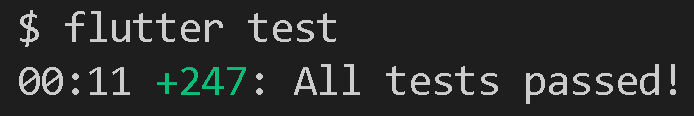
\includegraphics[width=0.8\textwidth]{figuras/cap5/5_tests_result.png}
  \caption{Resultado dos testes unitários da aplicação Nurse.}
  \label{fig:tests_result}
\end{figure}

\begin{figure}[!ht]
  \centering
  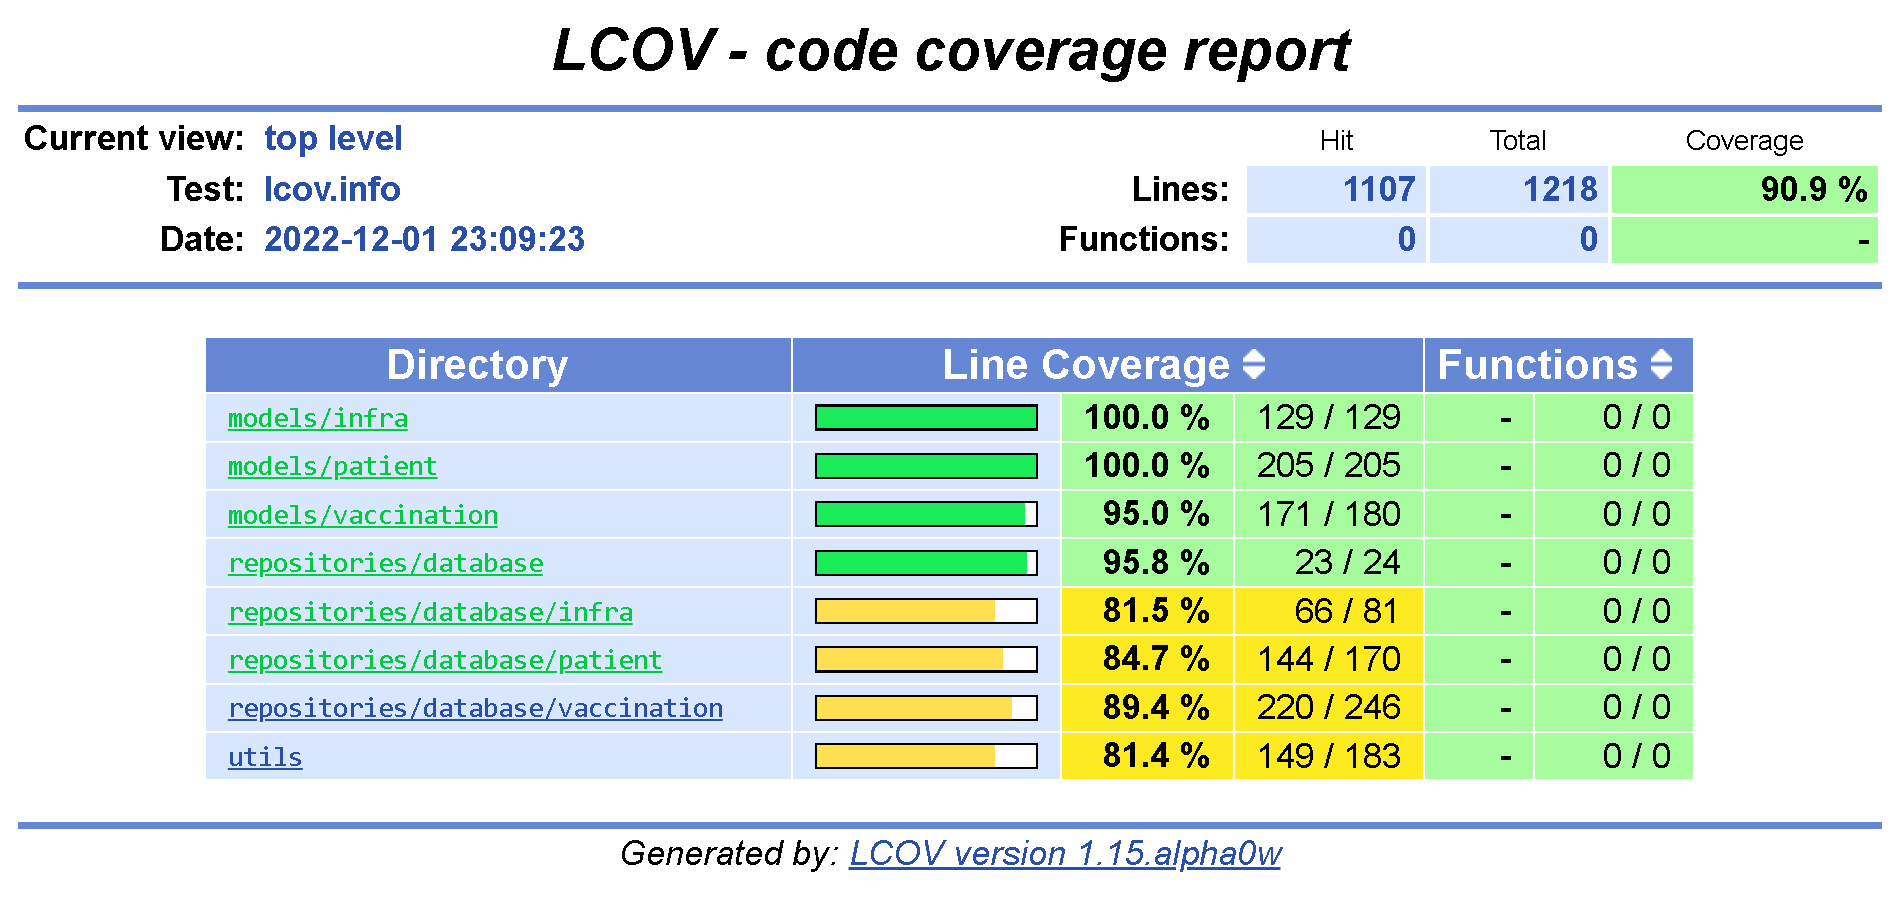
\includegraphics[width=\textwidth]{figuras/cap5/5_coverage_report.png}
  \caption{Cobertura de testes na aplicação Nurse}
  \label{fig:tests_coverage}
\end{figure}

Para a realização dos testes unitários, utilizou-se um dos pacotes nativos do \textit{framework Flutter}, chamado \textit{flutter\_test}, que foi adicionado como uma das dependências de desenvolvimento da aplicação. Então, criou-se um arquivos de testes para cada classe relacionada aos modelos da aplicação e aos seus repositórios. Para cada um dessas classes, foram criados testes unitários para verificar se as funções públicas estão realizando o que se espera delas. E, para rodar os testes, bastou executar o comando \textit{flutter test} no terminal.

Já para verificação de cobertura de testes do código, utilizou-se a flag \textit{--coverage} no comando de testes, o que forneceu um relatório de cobertura de código. Em posse desse relatório e utilizando-se da ferramenta \textit{lcov}, foi possível gerar uma página HTML (do inglês, \textit{HyperText Markup Language}) com a visão geral da cobertura dos testes, como mostrado na Figura \ref{fig:tests_coverage} e com os detalhes de cada arquivo com código associado \cite{lcov}.

% \section{Testes de Performance}
% \label{cap5:Sec:TestesPerformance}
% [A fazer] [Feito]{Não adicionado}{Buscar os métodos de testes de performance do Flutter e do Dart.}

\section{Fluxos de Telas}
\label{cap5:Sec:FluxosTelas}
As seções mostradas a seguir representam os principais fluxos de telas da aplicação Nurse. A primeira seção apresenta o fluxo de telas para o cadastro de uma nova entidade, como um paciente ou uma vacina, por exemplo. A segunda seção também apresenta o cadastro de uma entidade, mas a vacinação é a entidade central da aplicação e possui um fluxo ligeiramente diferente das demais entidades. A seção seguinte mostra o fluxo para uma edição de entidade e, por fim, a última seção compreende o fluxo de telas para a geração e exportação de uma planilha de vacinações em um dado período. 

\subsection{Fluxo de cadastro de entidade}
\label{cap5:SubSec:FluxoCadastroEntidade}
O fluxo de cadastro de entidade é composto por três telas, sendo a primeira tela responsável por apresentar a lista de tipos de entidade presentes na aplicação (Aplicante, Vacina, Lote de Vacina...). Ao selecionar uma dessas opções, uma lista com todos os cadastros individuais dessa entidade é apresentada na segunda tela. Por fim, na última tela, o usuário terá um formulário com os campos obrigatórios e opcionais para o cadastro da entidade selecionada e um botão de salvamento.

\begin{figure}[ht!]
  \centering
          \subfloat[Tela \textbf{Lista dos tipos de entidade}]{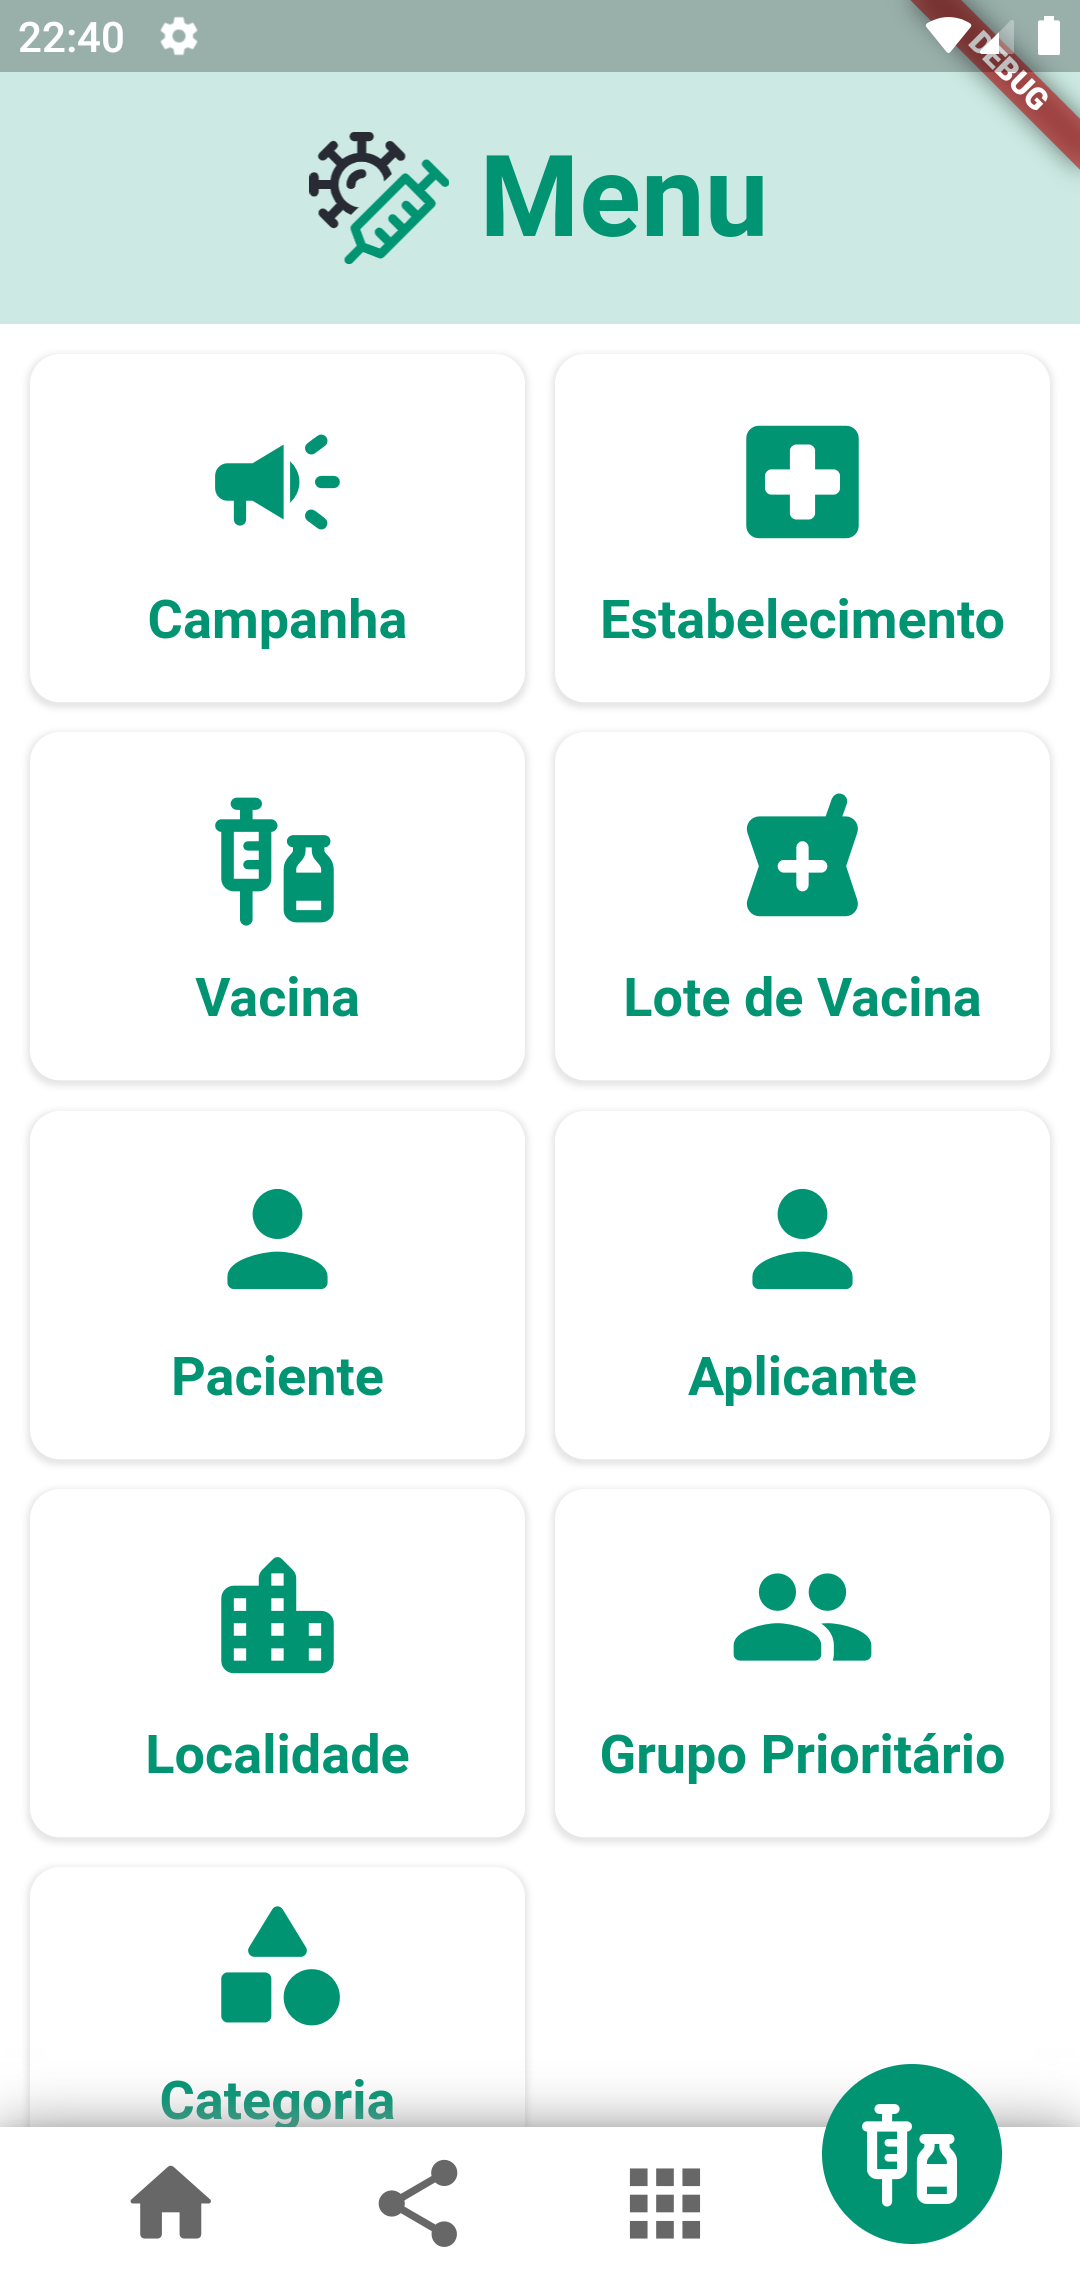
\includegraphics[width=0.29\columnwidth]{figuras/cap4/4_2_entities_screen.png}}
            \qquad
          \subfloat[Tela \textbf{Lista das campanhas cadastradas}]{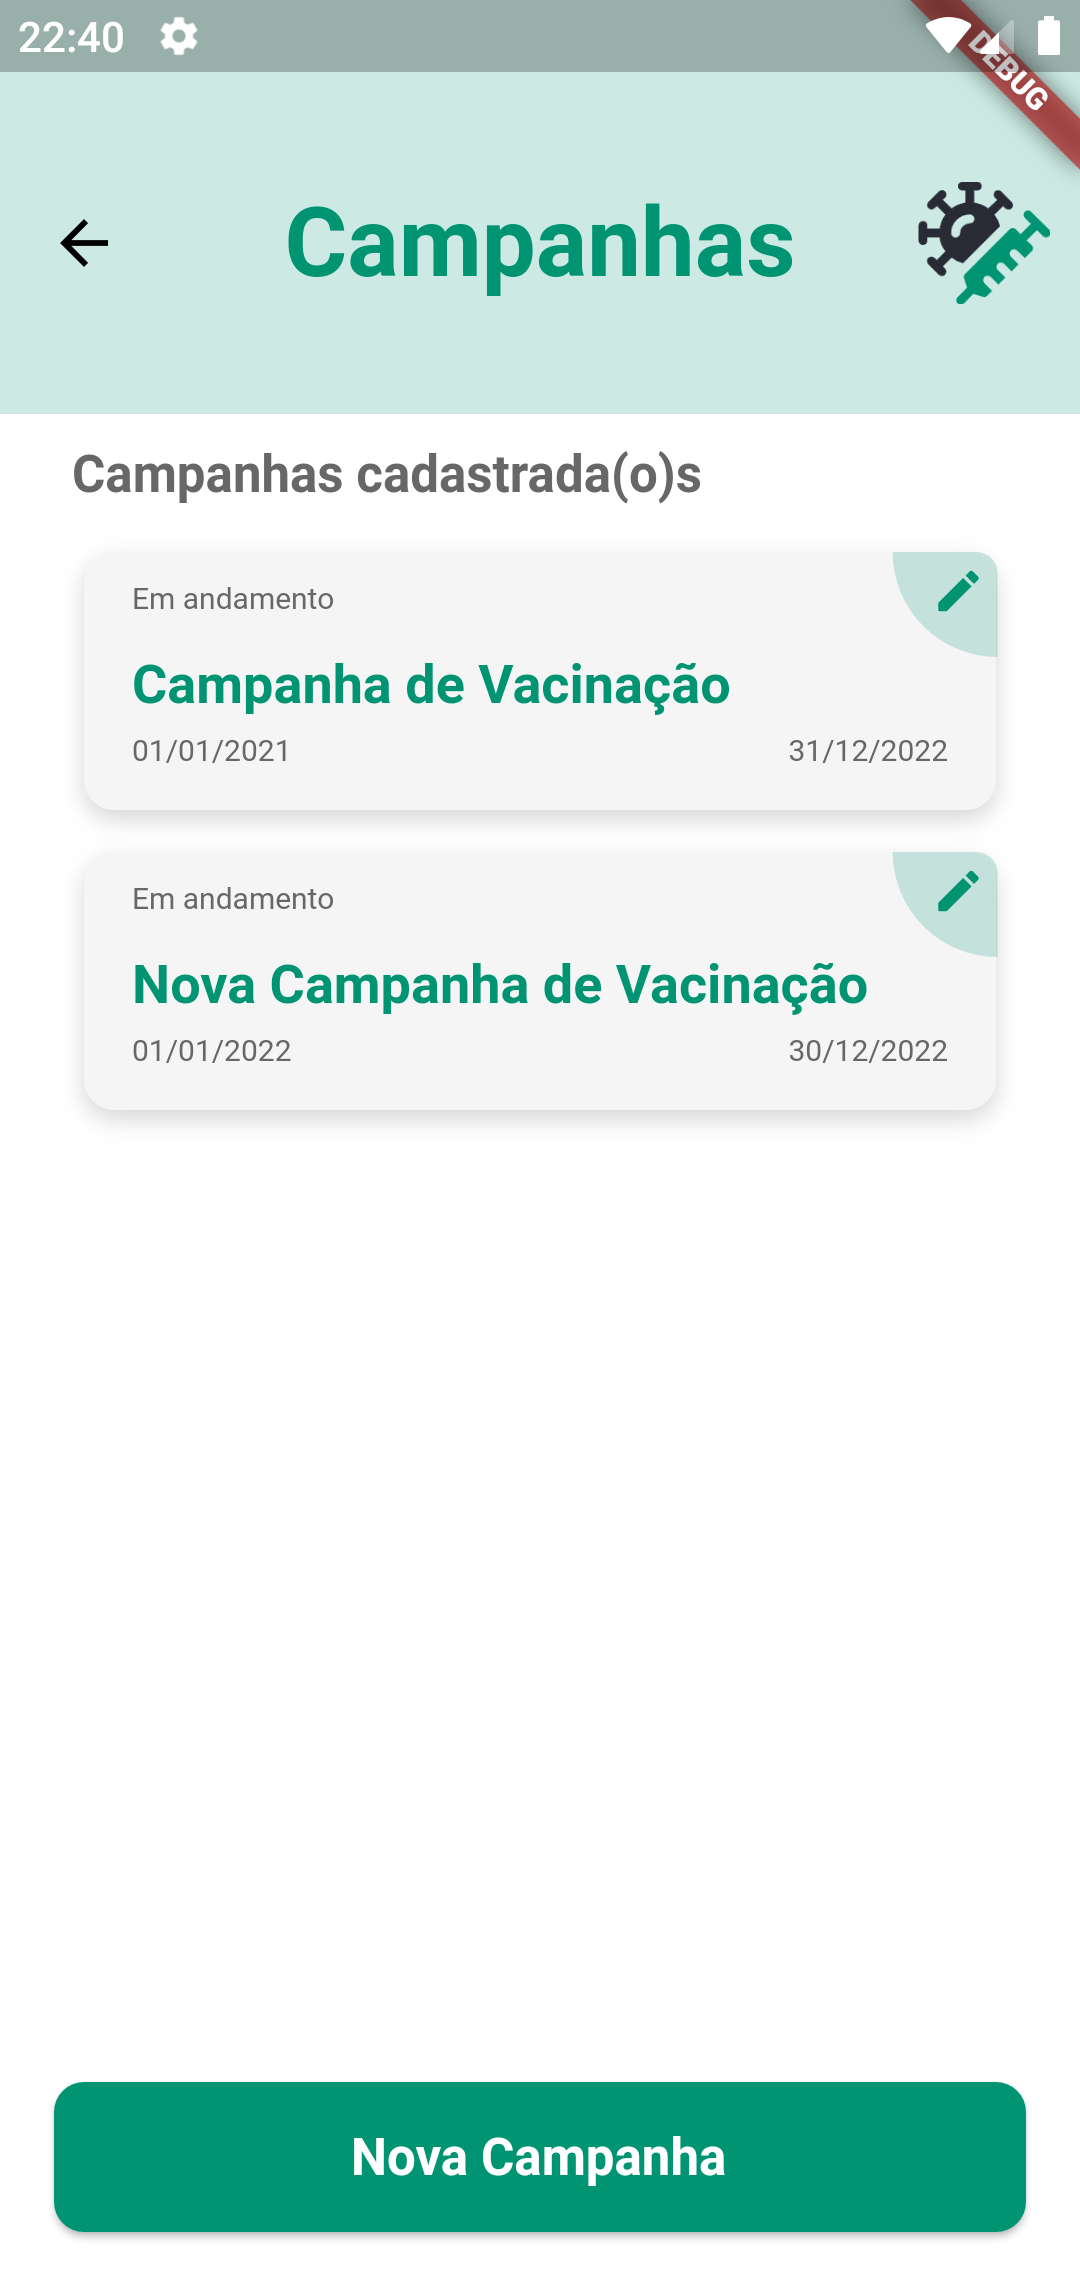
\includegraphics[width=0.29\columnwidth]{figuras/cap4/4_2_campaign_list_screen.png}}
            \qquad
          \subfloat[Tela \textbf{Formulário de cadastro de campanha}]{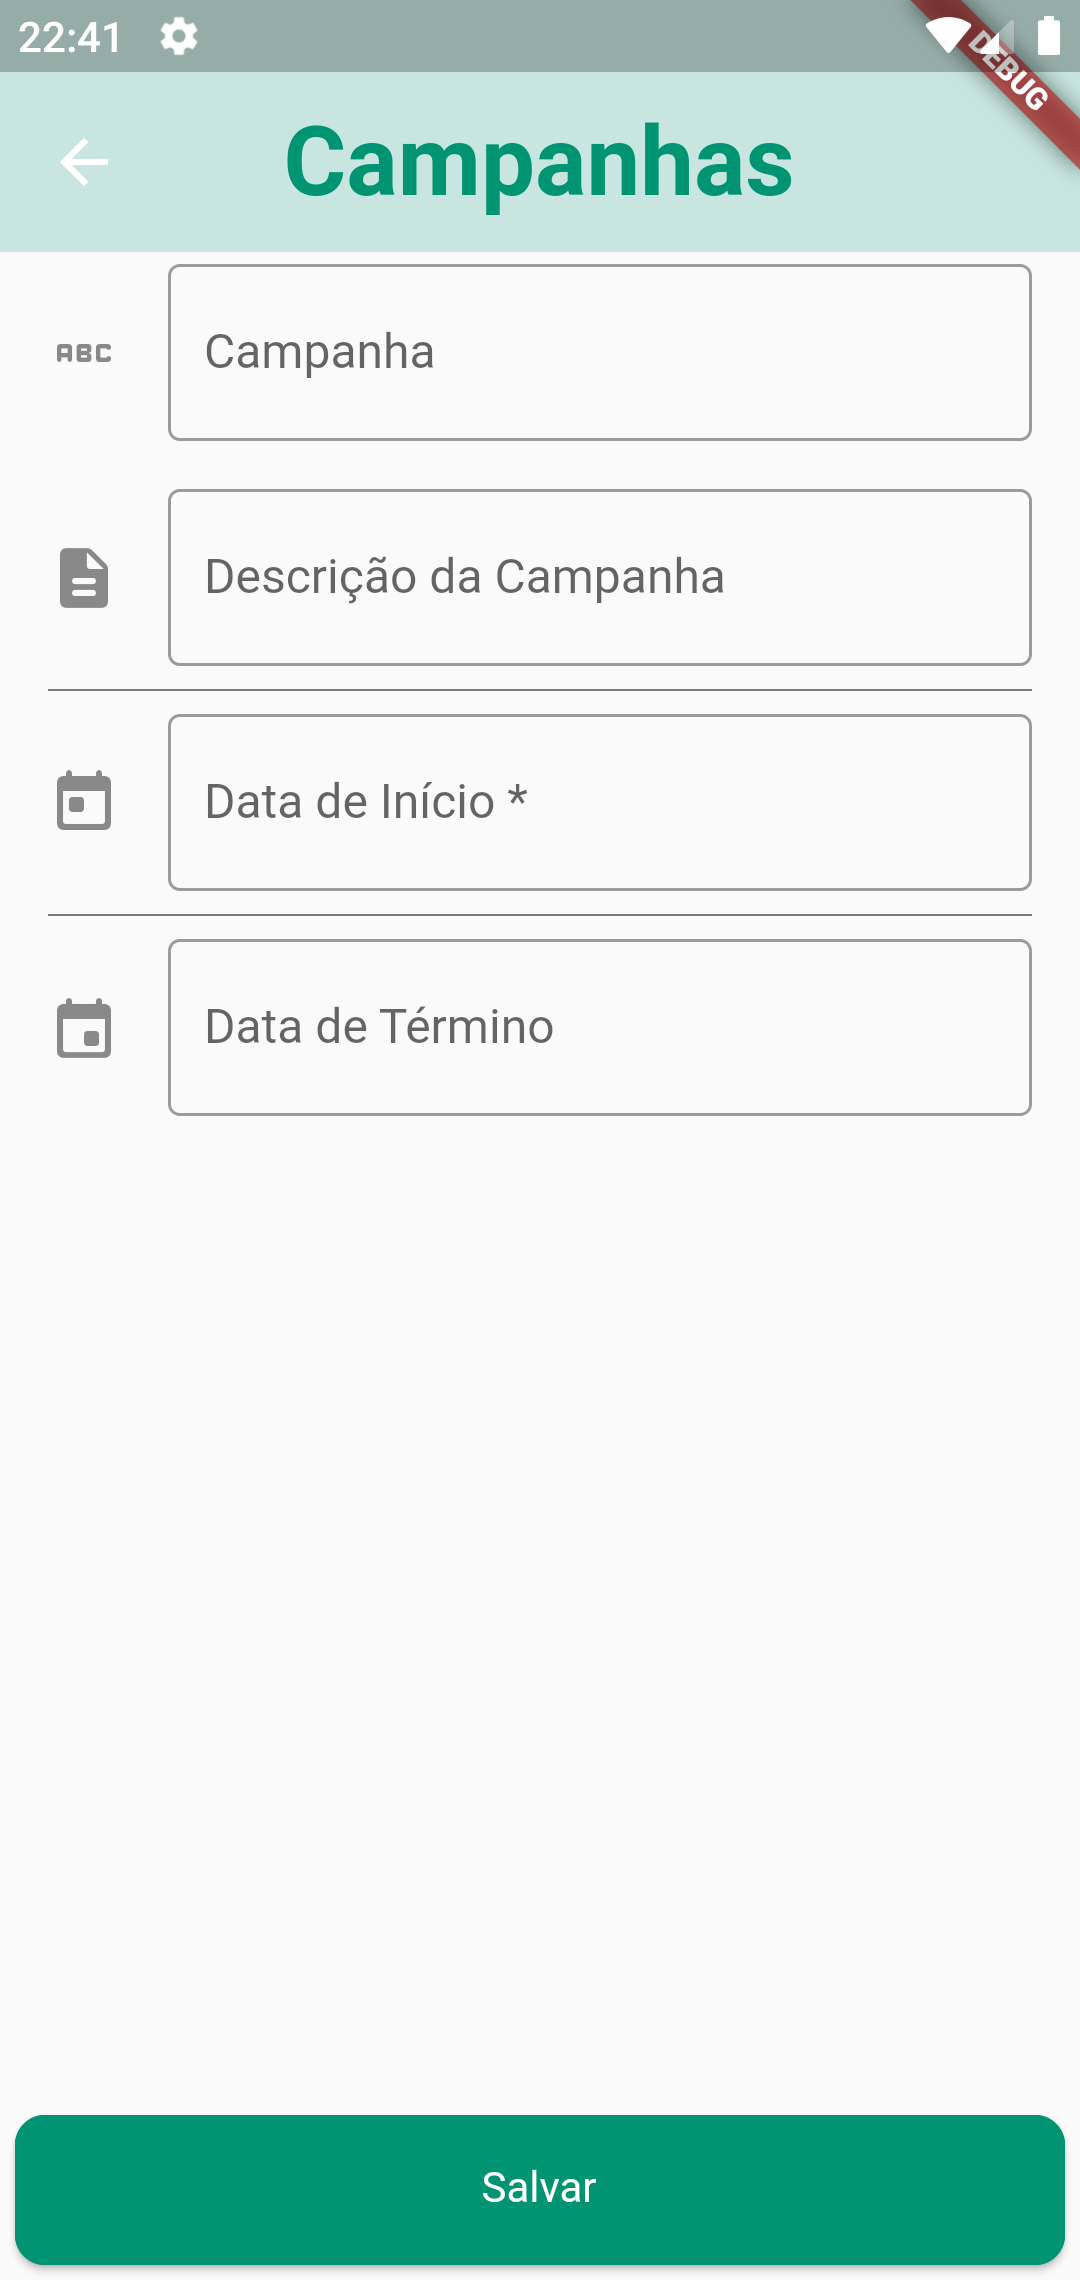
\includegraphics[width=0.29\columnwidth]{figuras/cap4/4_2_campaign_form.png}}
    \caption[Fluxo de cadastro de nova campanha (parte 1)]{Fluxo de cadastro de nova campanha (parte 1)}
  % \fonte{Inserir autor aqui}
  
  \label{fig:new_campaign_flux_1}
\end{figure}

Caso haja algum erro de validação dos campos, o usuário será informado por meio de uma mensagem de erro que aparecerá logo abaixo do campo ao qual o erro se refere. Com o fomulário preenchido, o usuário poderá tentar salvar a nova entrada e, caso o salvamento seja bem sucedido, será redirecionado para a tela de listagem da entidade cadastrada. Caso contrário, será informado por meio de uma mensagem de erro que aparecerá no centro da tela, em um \textit{pop-up}.

\begin{figure}[ht!]
  \centering
      \subfloat[Tela \textbf{Formulário de cadastro de campanha com erro}]{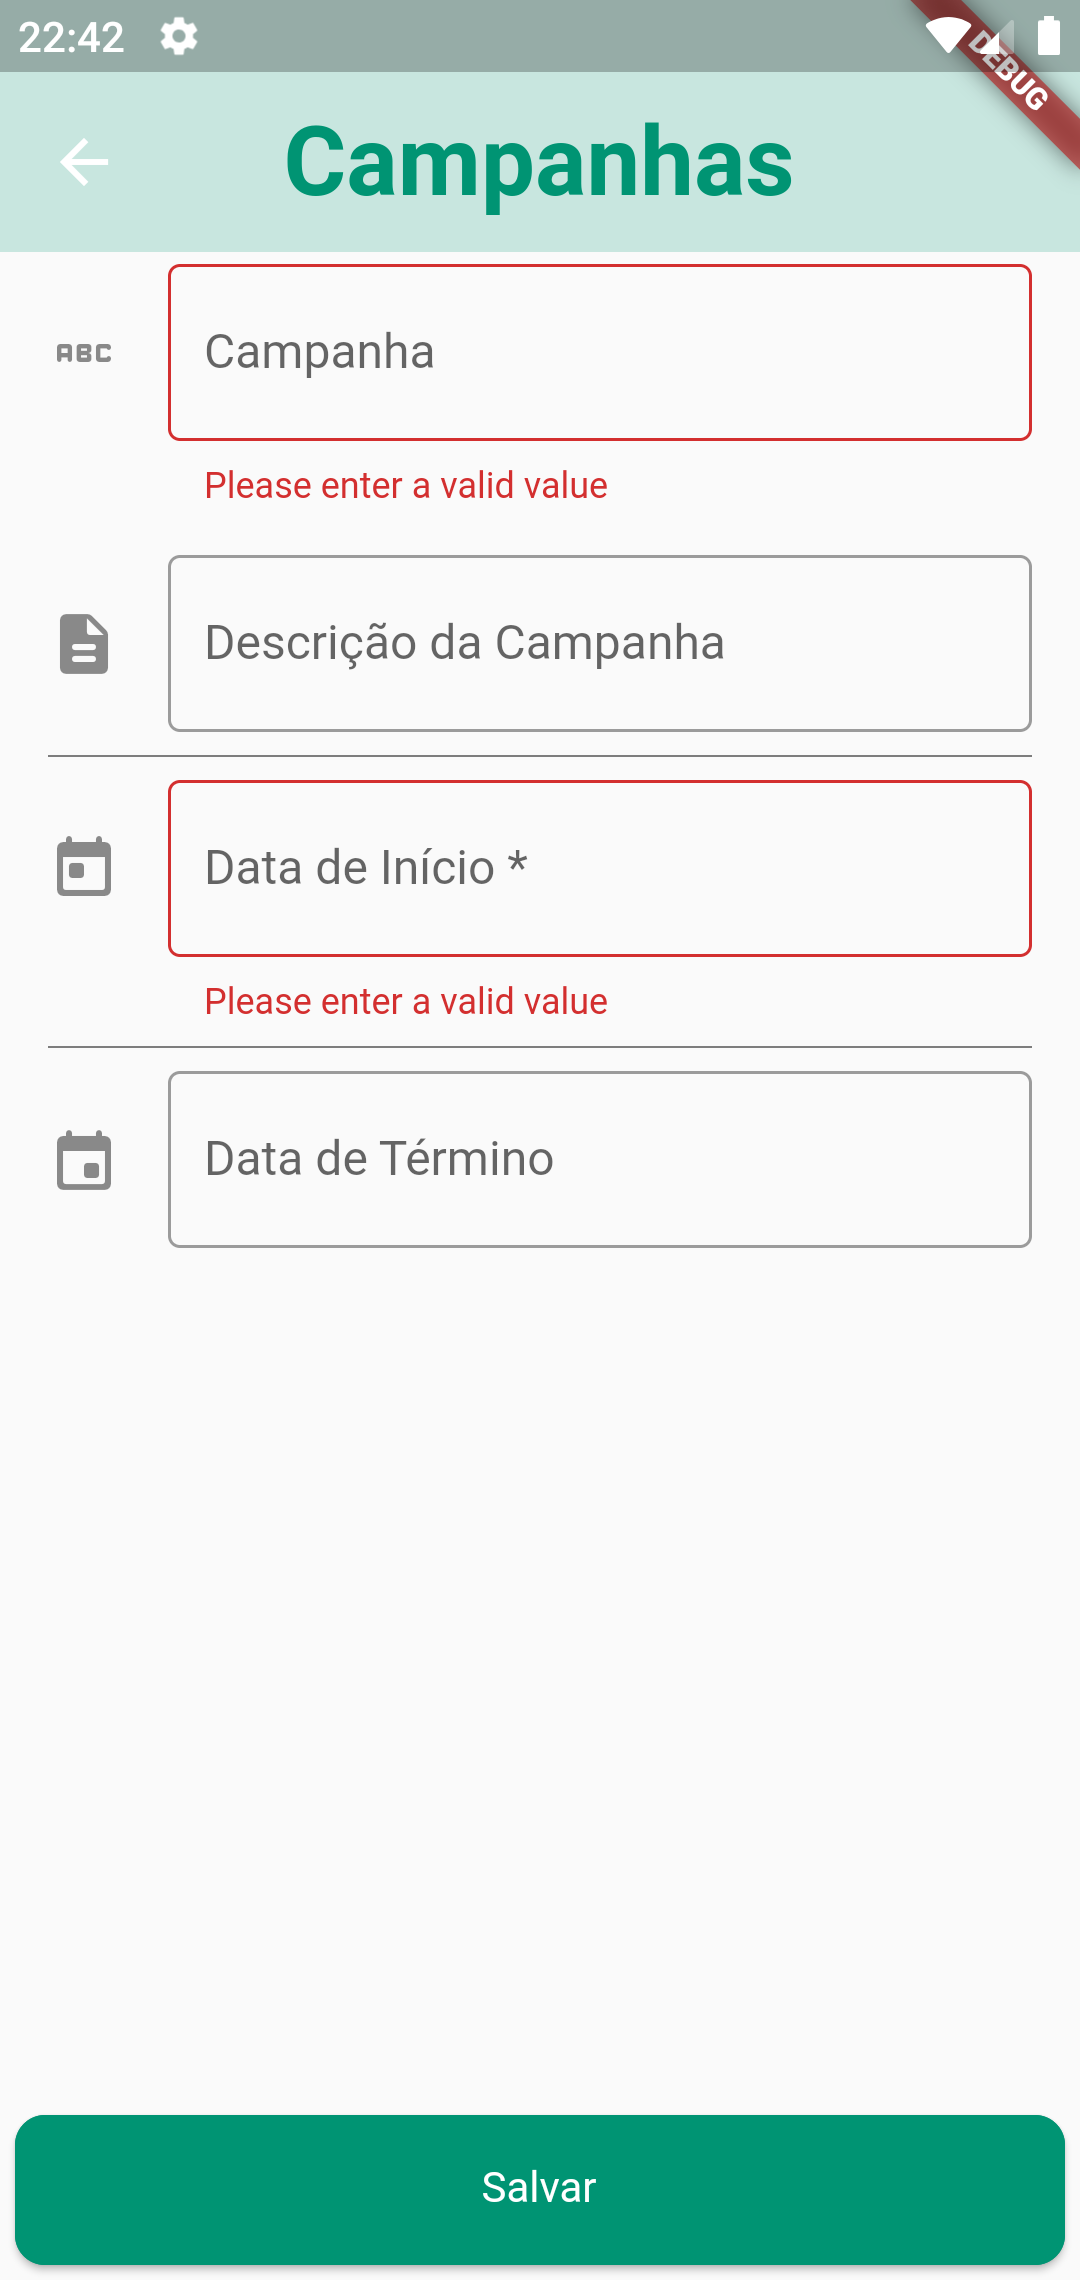
\includegraphics[width=0.29\columnwidth]{figuras/cap4/4_2_campaign_form_on_error.png}}
        \qquad
      \subfloat[Tela \textbf{Formulário de cadastro de campanha preenchido}]{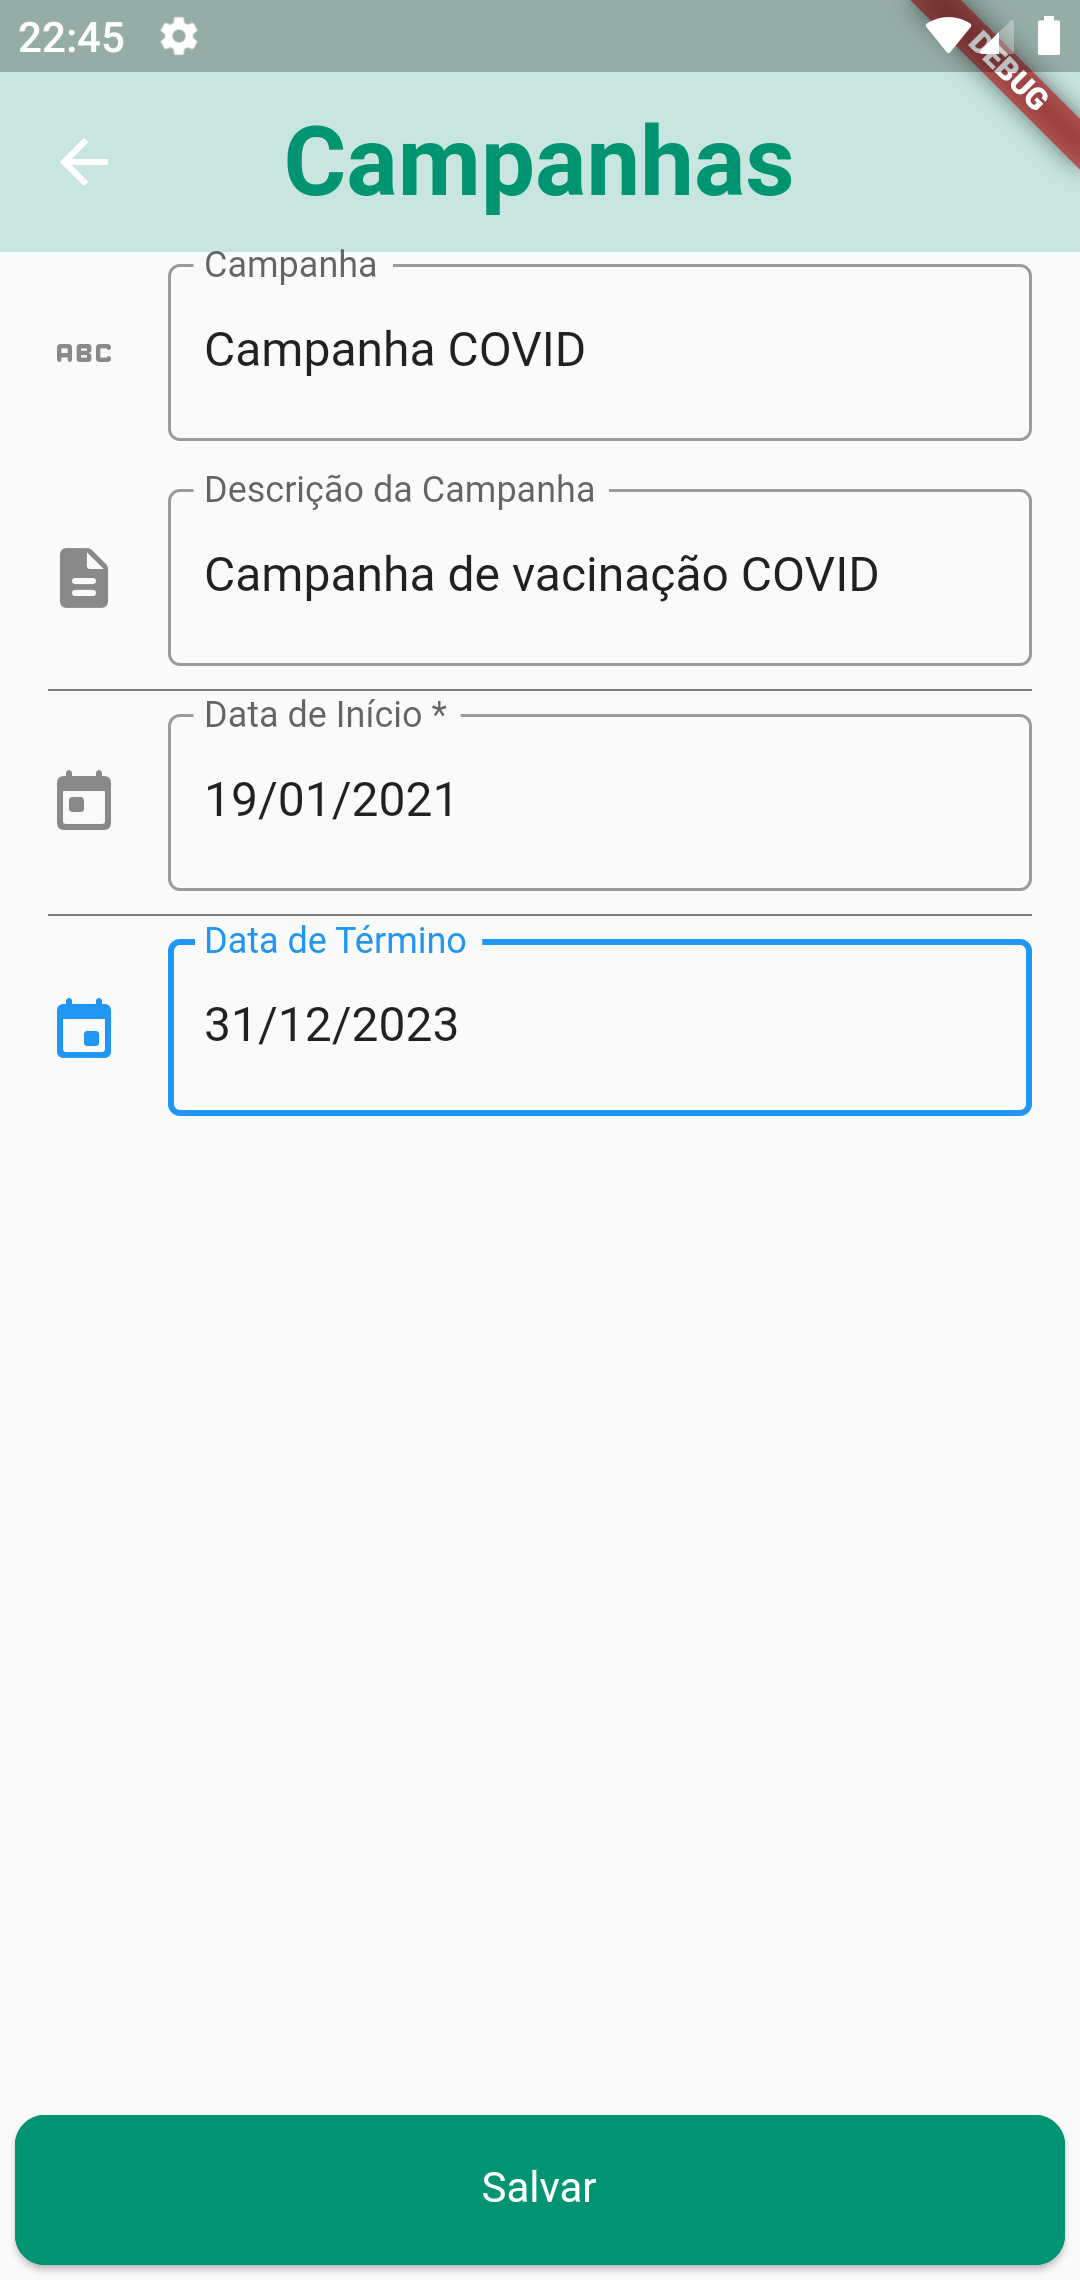
\includegraphics[width=0.29\columnwidth]{figuras/cap4/4_2_campaign_form_2.png}}
        \qquad
      \subfloat[Tela \textbf{Lista das campanhas após cadastro}]{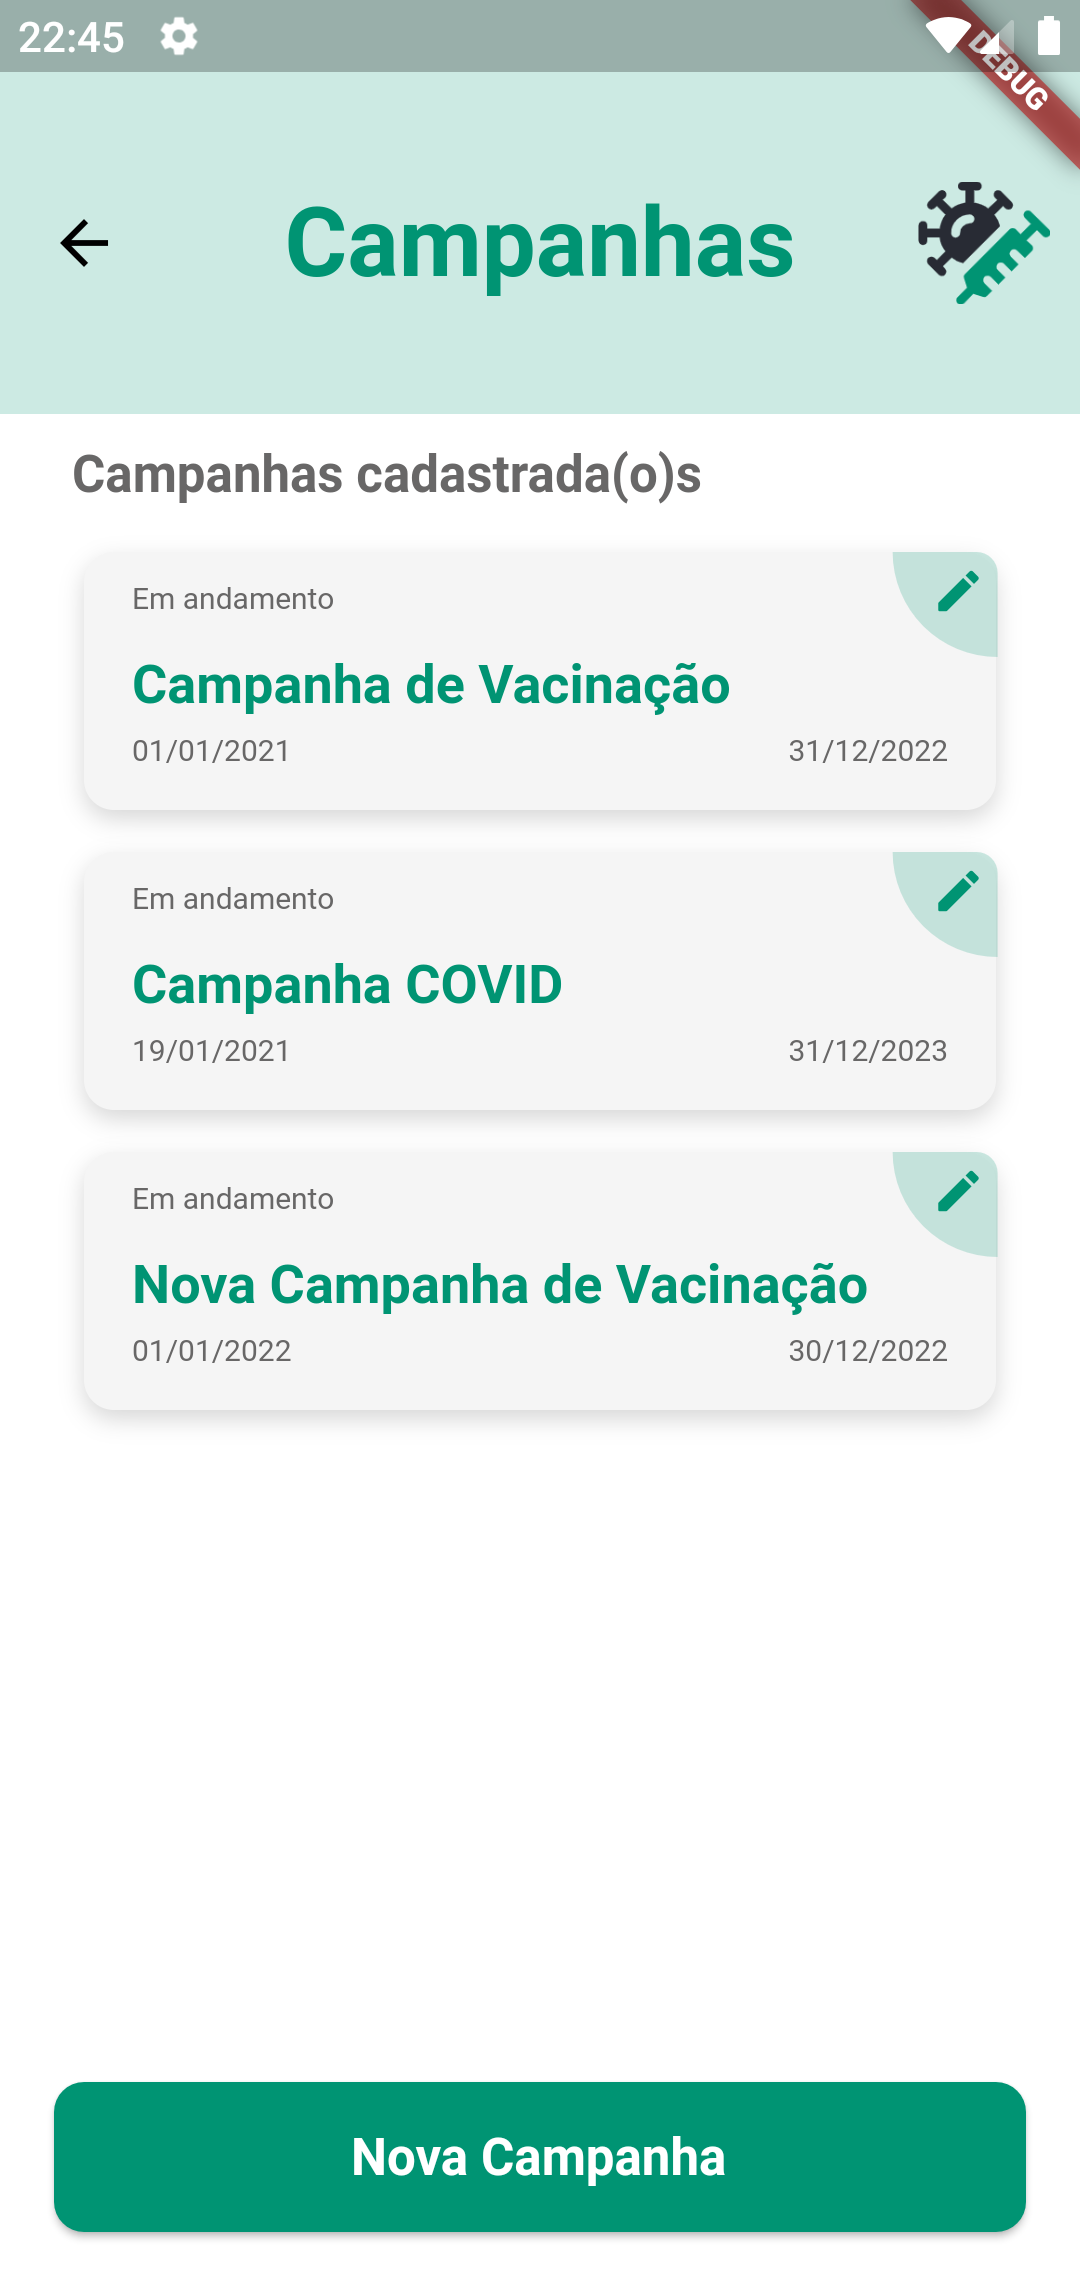
\includegraphics[width=0.29\columnwidth]{figuras/cap4/4_2_campaign_list_screen_2.png}}
    \caption[Fluxo de cadastro de nova campanha (parte 2)]{Fluxo de cadastro de nova campanha (parte 2)}
  % \fonte{Inserir autor aqui}
  
  \label{fig:new_campaign_flux_2}
\end{figure}

Vale ressaltar que parte do fluxo de cadastro de uma nova campanha foi apresentado na seção \ref{cap4:Sec:Telas}, Figura \ref{fig:entity_list_new_entity}. Sendo assim, o exemplo apresentado nessa seção (Figuras \ref{fig:new_campaign_flux_1} e \ref{fig:new_campaign_flux_2}) é semelhante àquele, assim como às demais telas de cadastro de entidades. A exceção é a tela de cadastro de uma nova vacinação, que será apresentada a seguir, na seção \ref{cap5:SubSec:FluxoCadastroVacinacao}.

\subsection{Fluxo de cadastro de vacinação}
\label{cap5:SubSec:FluxoCadastroVacinacao}
Como essa é uma entidade que engloba todas as outras, seu formulário é mais extenso e, por conta disso, decidiu-se subdividir esse formulário em mais partes. Além disso, o formulário é acessado não pela listagem de entidades, mas por meio de um botão de destaque presente na barra de navegação da aplicação.

O fluxo inicia-se nesse ponto, quando o usuário aperta no botão com o símbolo da aplicação. Em seguida, é exibido um formulário com múltiplas páginas e dois botões na parte inferior da tela para navegação entre as páginas. Na última página o botão de salvar aparece e o usuário pode salvar o novo registro de vacinação, seguindo as regras de preenchimento apresentadas na seção anterior (seção \ref{cap5:SubSec:FluxoCadastroEntidade}).

Ao fim do cadastro, o usuário é redirecionado à tela \textbf{Home}, onde será possível ver a nova vacinação cadastrada na lista de vacinações e os cartões com a contagem de doses aplicadas aumentar.

As Figuras \ref{fig:new_vaccination_flux_1} e \ref{fig:new_vaccination_flux_2} apresentam o fluxo descrito acima.

\begin{figure}[ht!]
  \centering
          \subfloat[\textbf{Botão para formulário de vacinação em destaque na barra de navegação}]{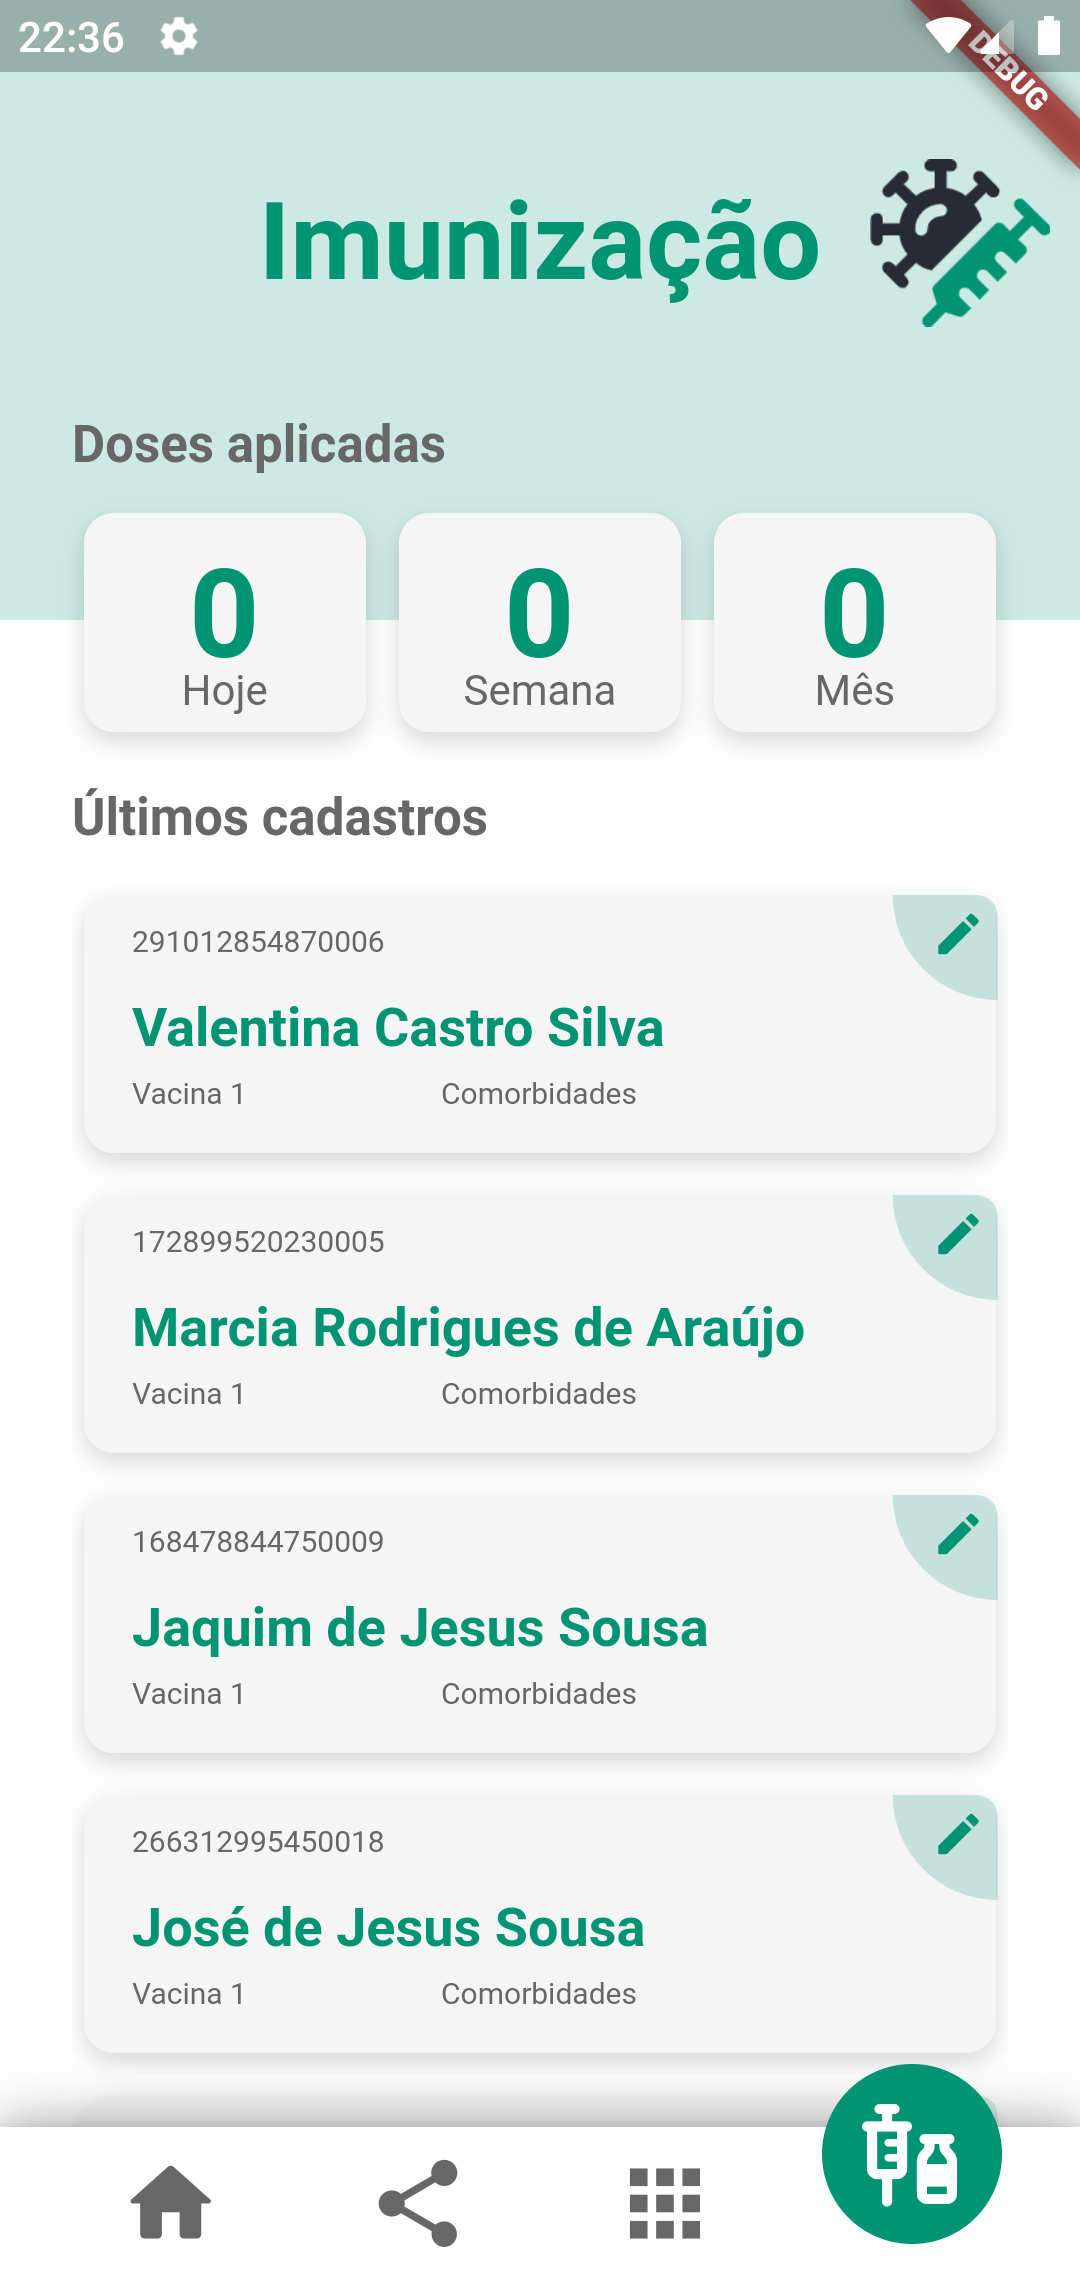
\includegraphics[width=0.29\columnwidth]{figuras/cap4/4_2_home_screen.png}}
            \qquad
          \subfloat[\textbf{Primeira tela do formulário}]{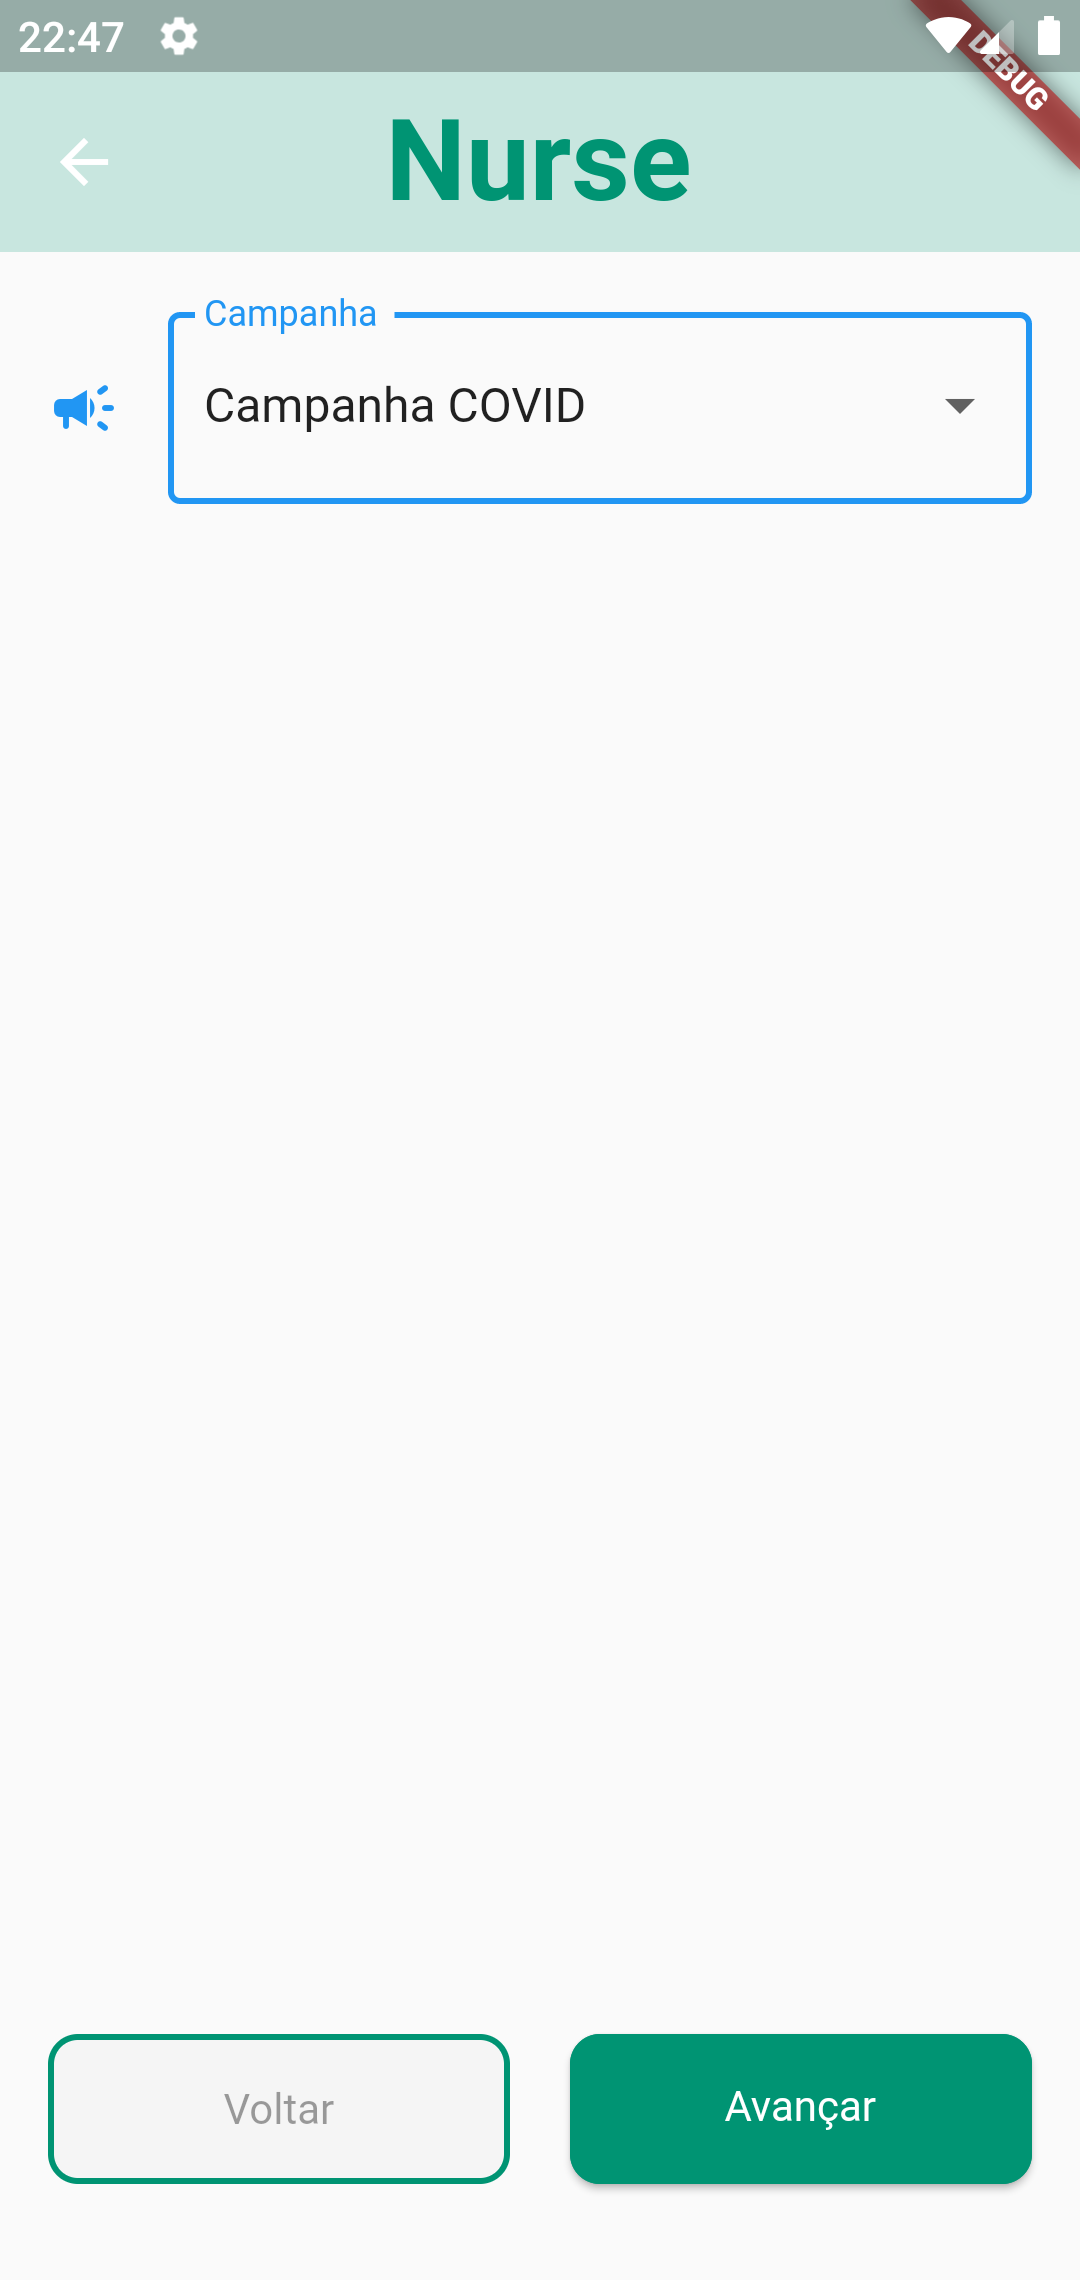
\includegraphics[width=0.29\columnwidth]{figuras/cap4/4_2_vaccination_campaign_form_2.png}}
            \qquad
          \subfloat[\textbf{Última tela do formulário}]{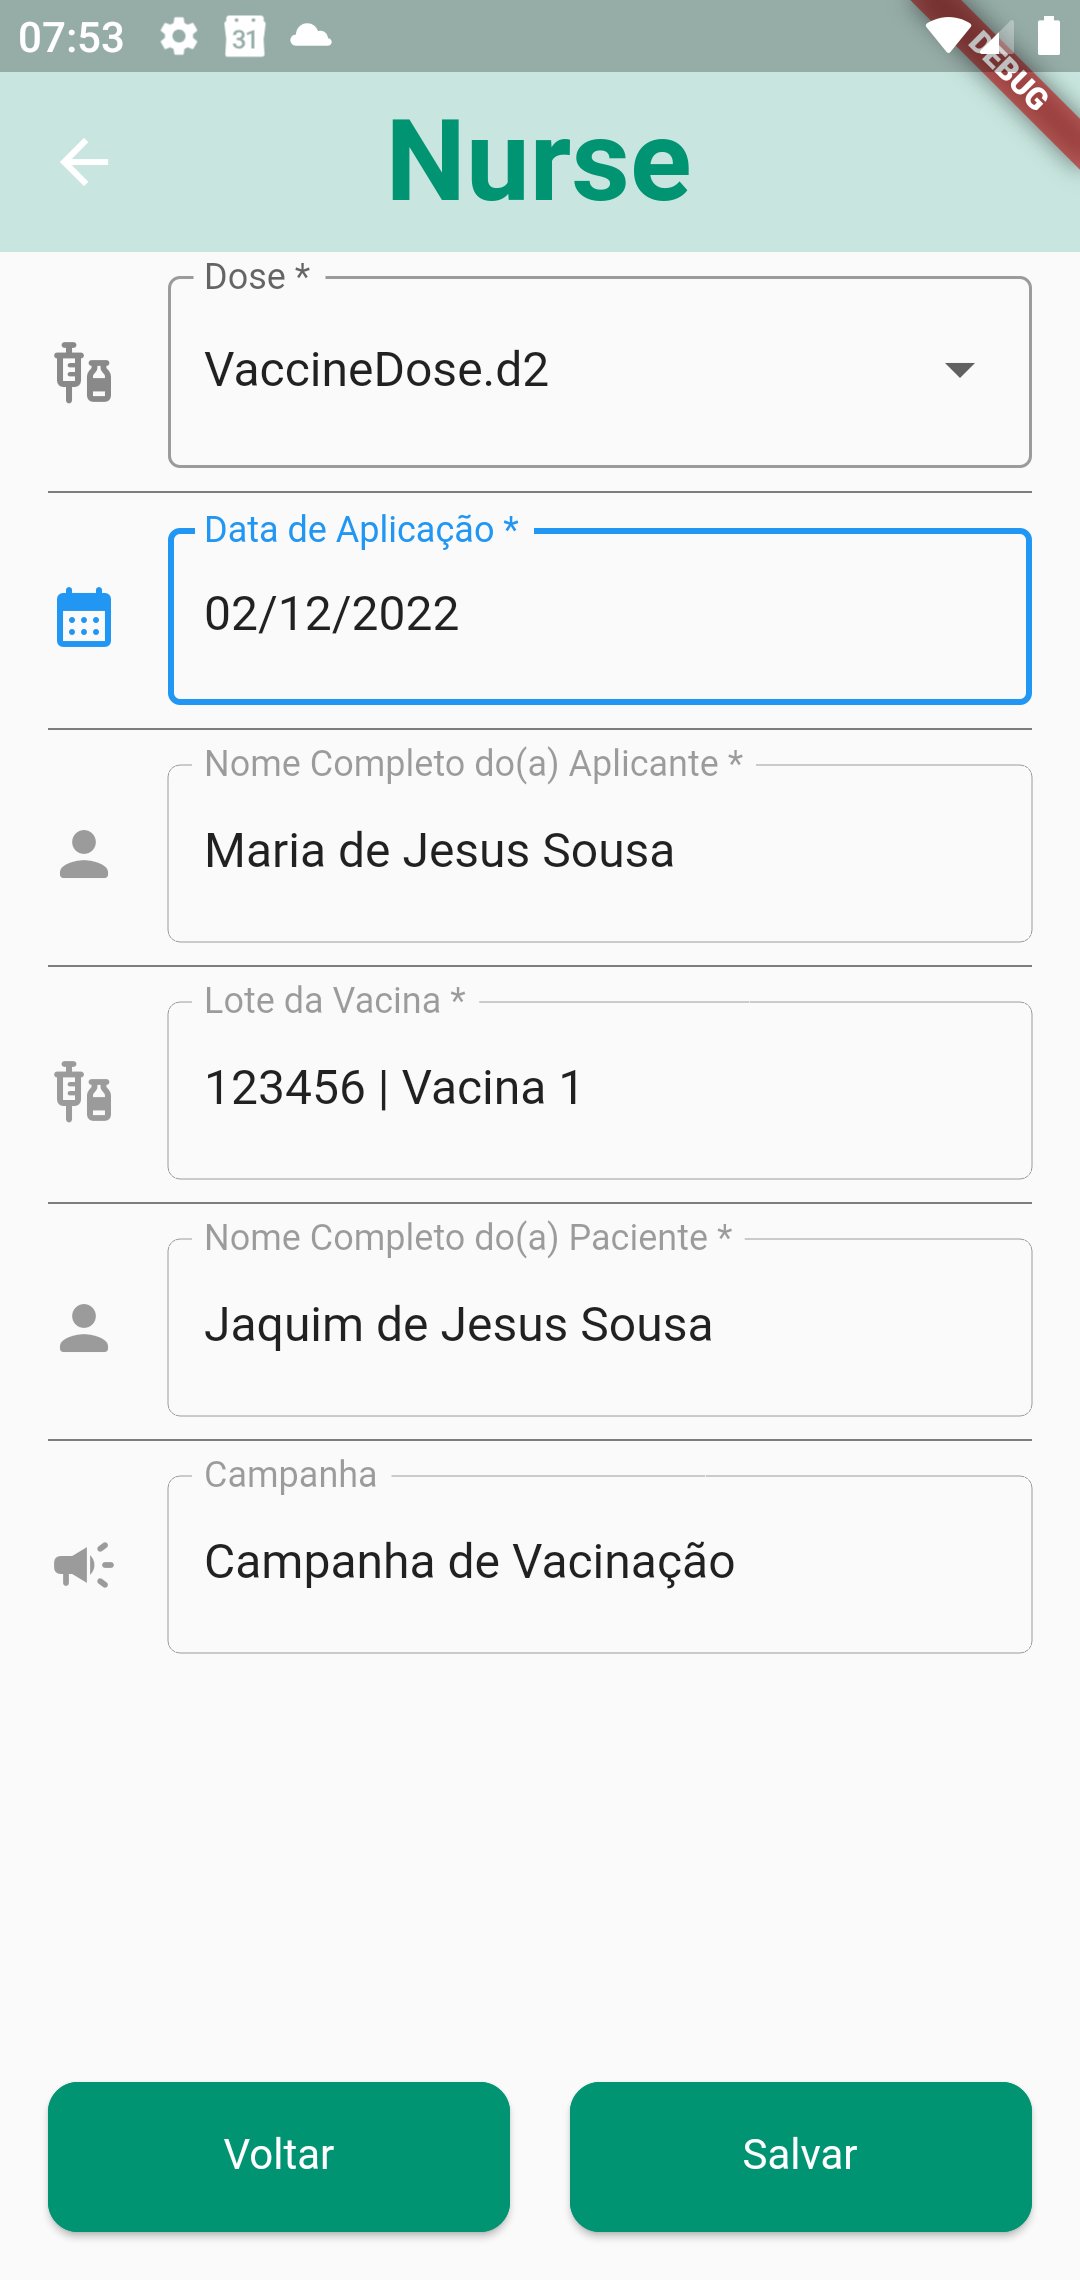
\includegraphics[width=0.29\columnwidth]{figuras/cap4/4_2_vaccination_overview_form.png}}
    \caption[Fluxo de cadastro de nova vacinação (parte 1)]{Fluxo de cadastro de nova vacinação (parte 1)}
  % \fonte{Inserir autor aqui}
  
  \label{fig:new_vaccination_flux_1}
\end{figure}

\begin{figure}[ht!]
  \centering
          \subfloat[Tela \textbf{de erro por cadastro já existente}]{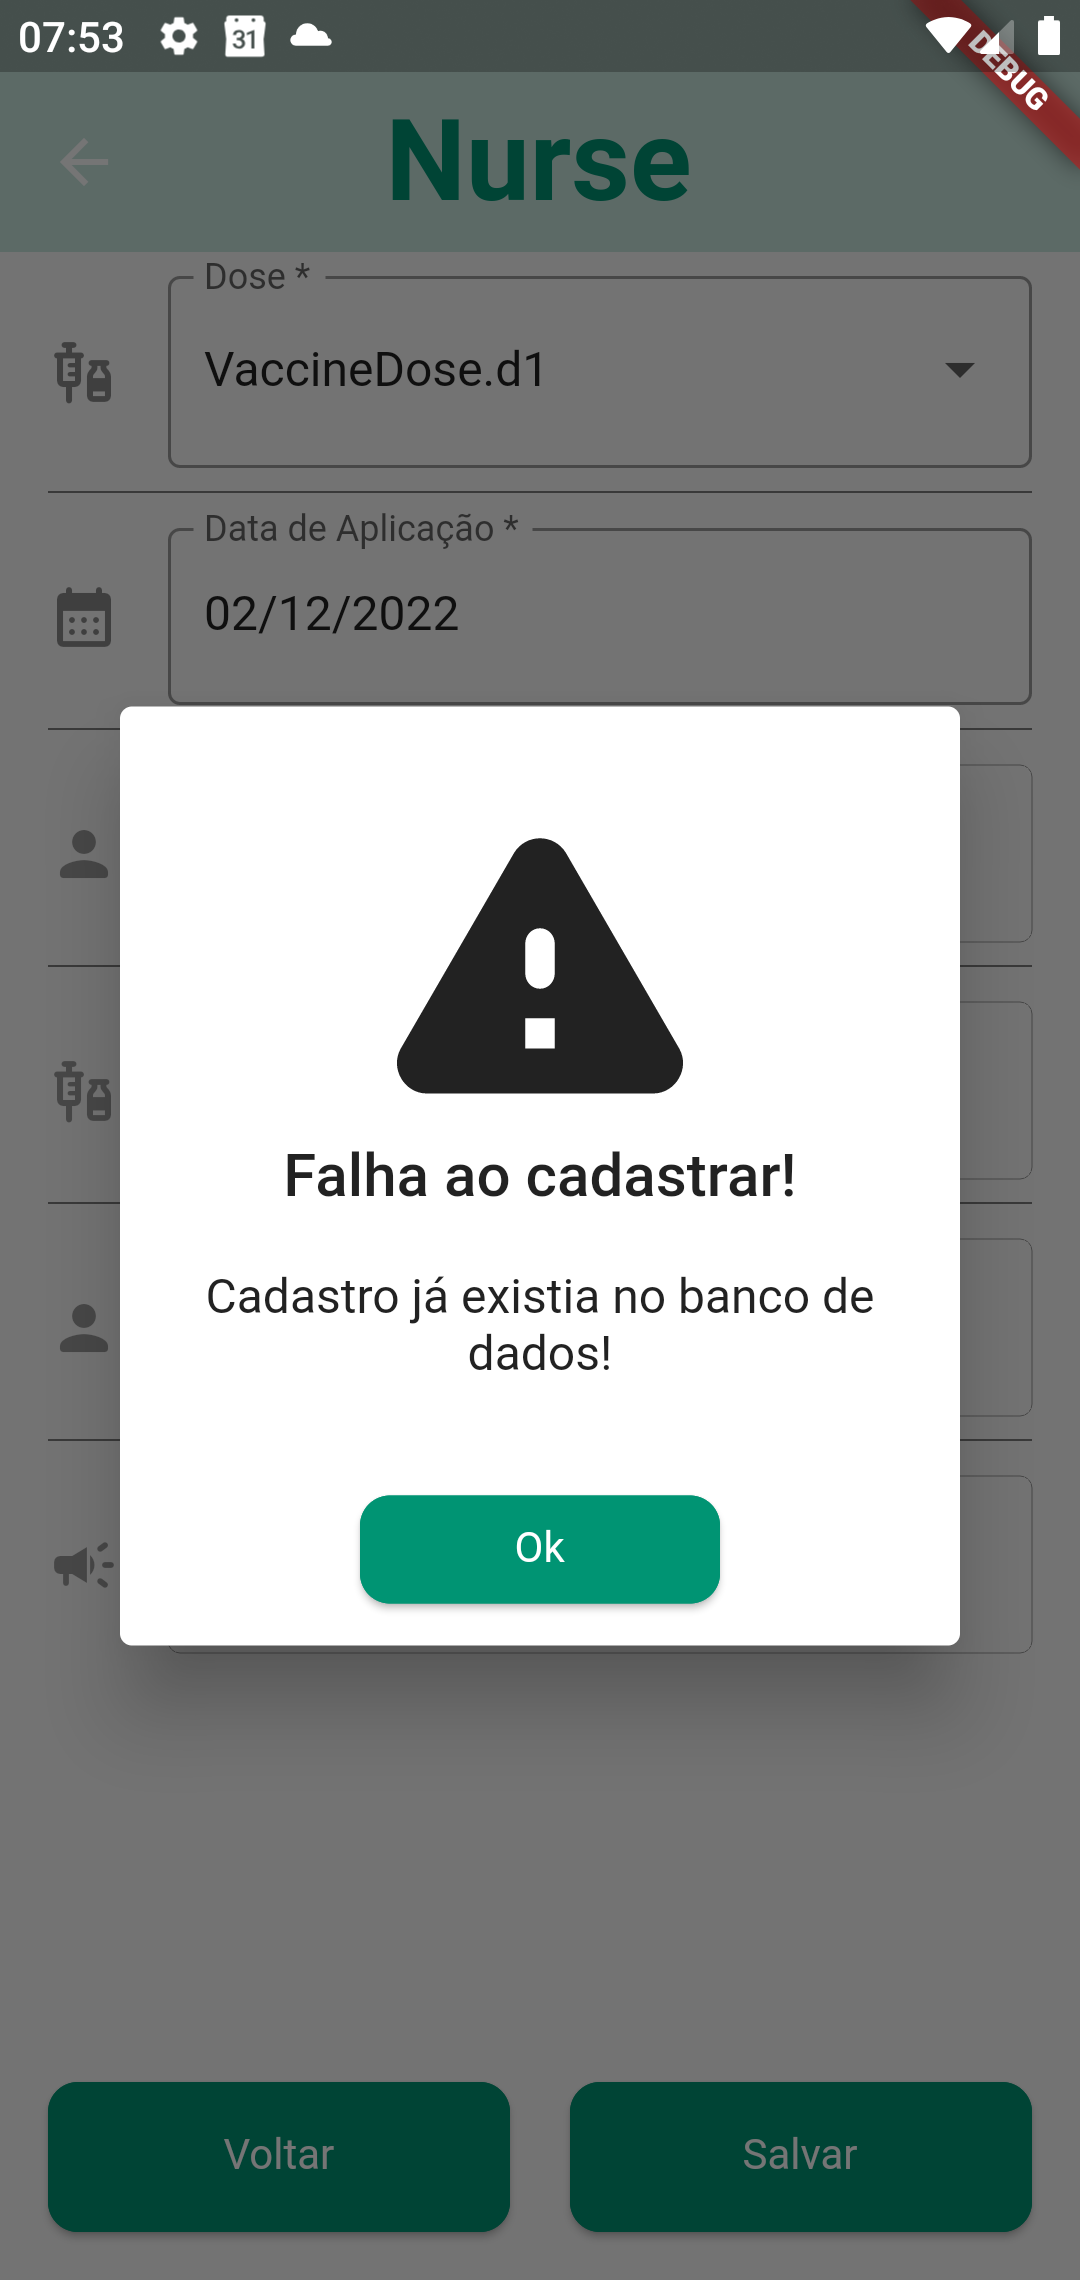
\includegraphics[width=0.29\columnwidth]{figuras/cap4/4_2_vaccination_on_form_error.png}}
            \qquad
          \subfloat[Tela \textbf{Home após cadastro de vacinação}]{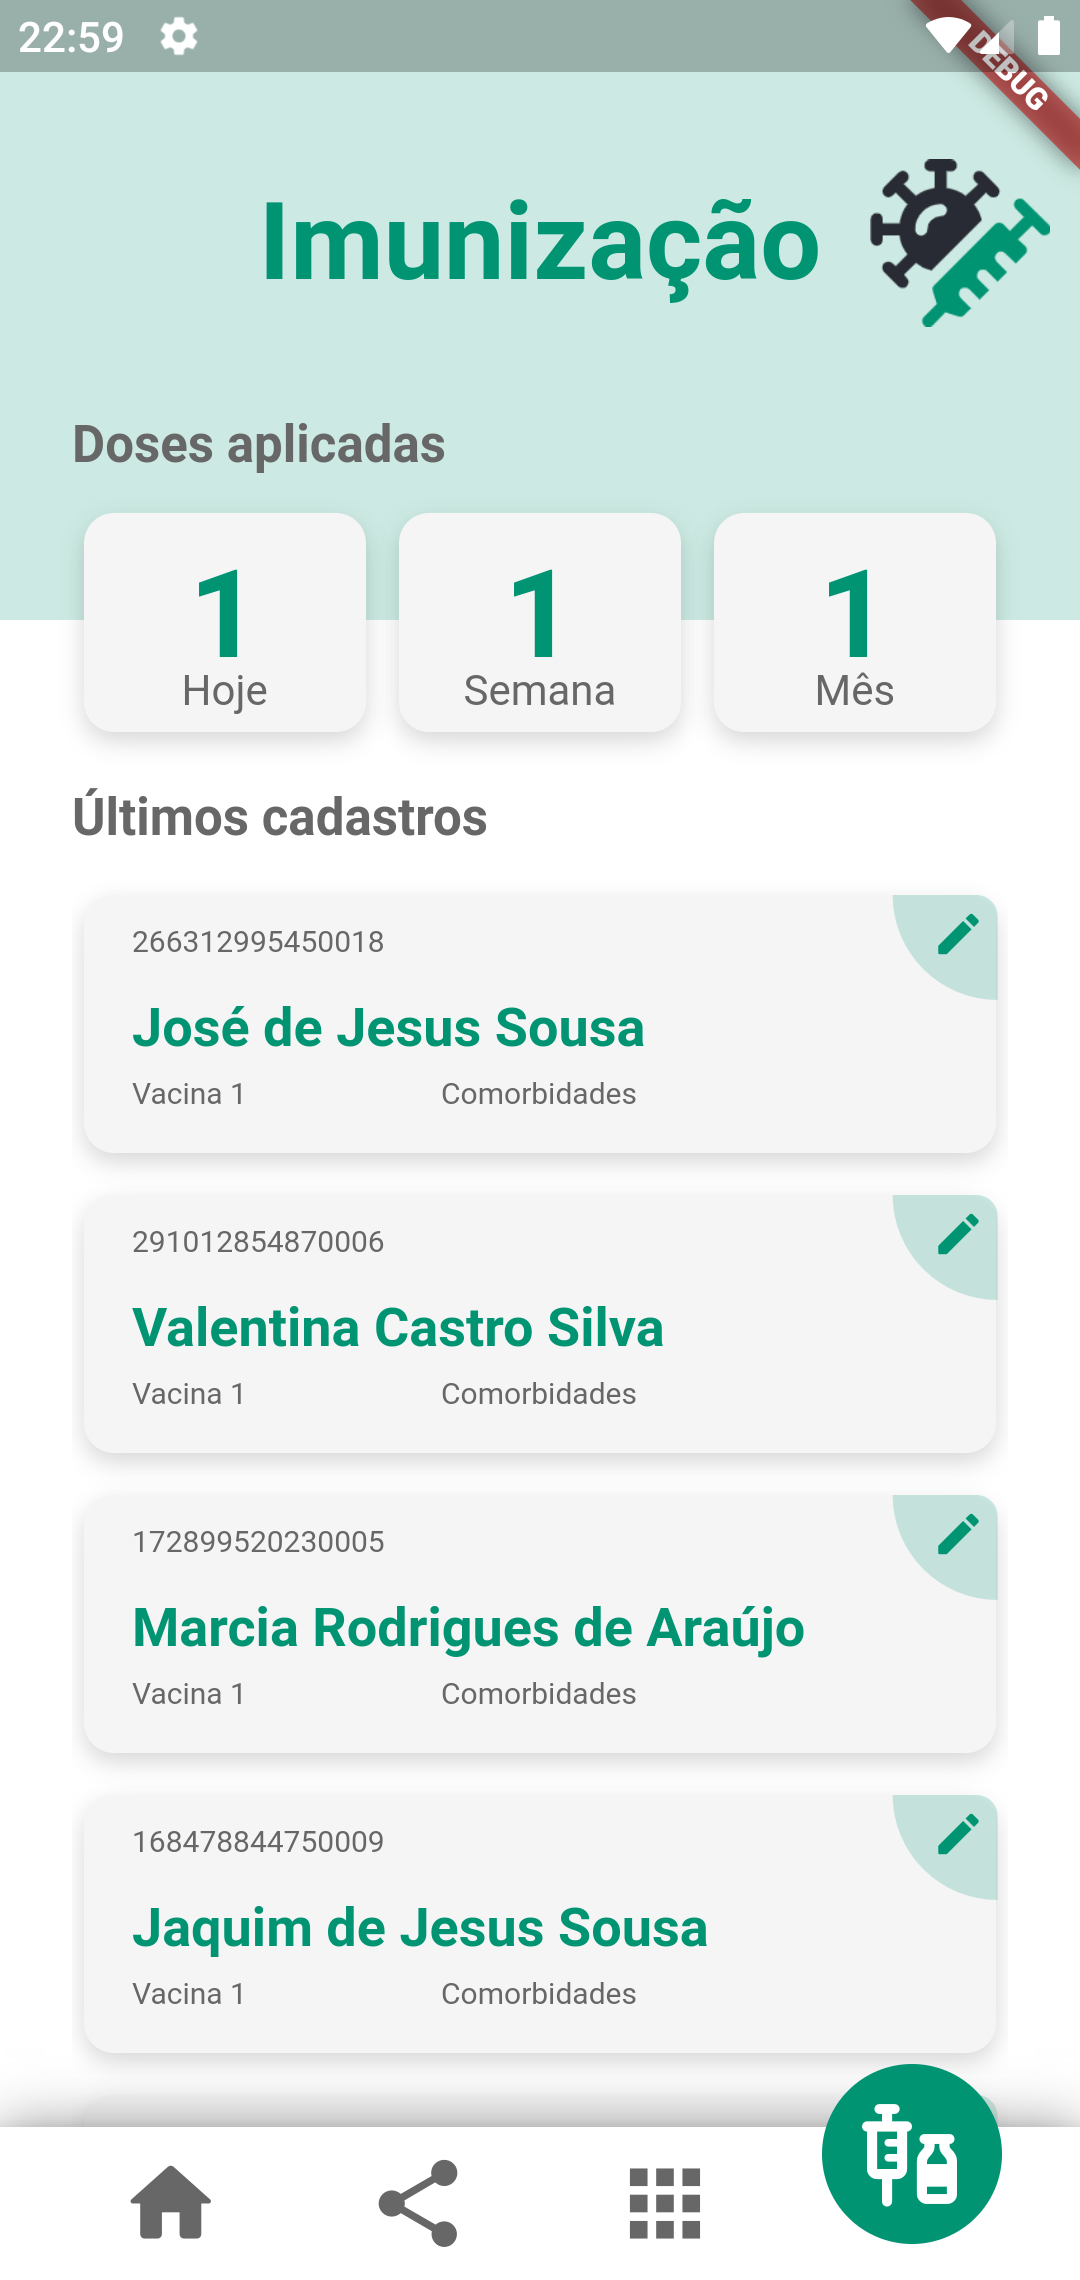
\includegraphics[width=0.29\columnwidth]{figuras/cap4/4_2_home_screen_2.png}}
    \caption[Fluxo de cadastro de nova vacinação (parte 2)]{Fluxo de cadastro de nova vacinação (parte 2)}
  % \fonte{Inserir autor aqui}
  
  \label{fig:new_vaccination_flux_2}
\end{figure}

\subsection{Fluxo de exportação}
\label{cap5:SubSec:FluxoExportacao}
O fluxo de exportação inicia-se na tela que pode ser acessada ao apertar no ícone de exportação, presente na barra de navegação da aplicação. Nessa tela, o usuário pode escolher o período que deseja buscar vacinações para exportação.

Assim que o período é escolhido no calendário, o botão de exportar é habilitado e, ao apertá-lo, duas opções são apresentadas: abrir o arquivo ou compartilhá-lo.

Esse fluxo é apresentado nas Figuras \ref{fig:export_flux_1} e \ref{fig:export_flux_2}.

\begin{figure}[ht!]
  \centering
          \subfloat[Tela \textbf{exportação inicialmente}]{
\includegraphics[width=0.29\columnwidth]{figuras/cap4/4_2_export_screen_1.png}}
            \qquad
          \subfloat[\textbf{Calendário 1 para escolha do período de exportação}]{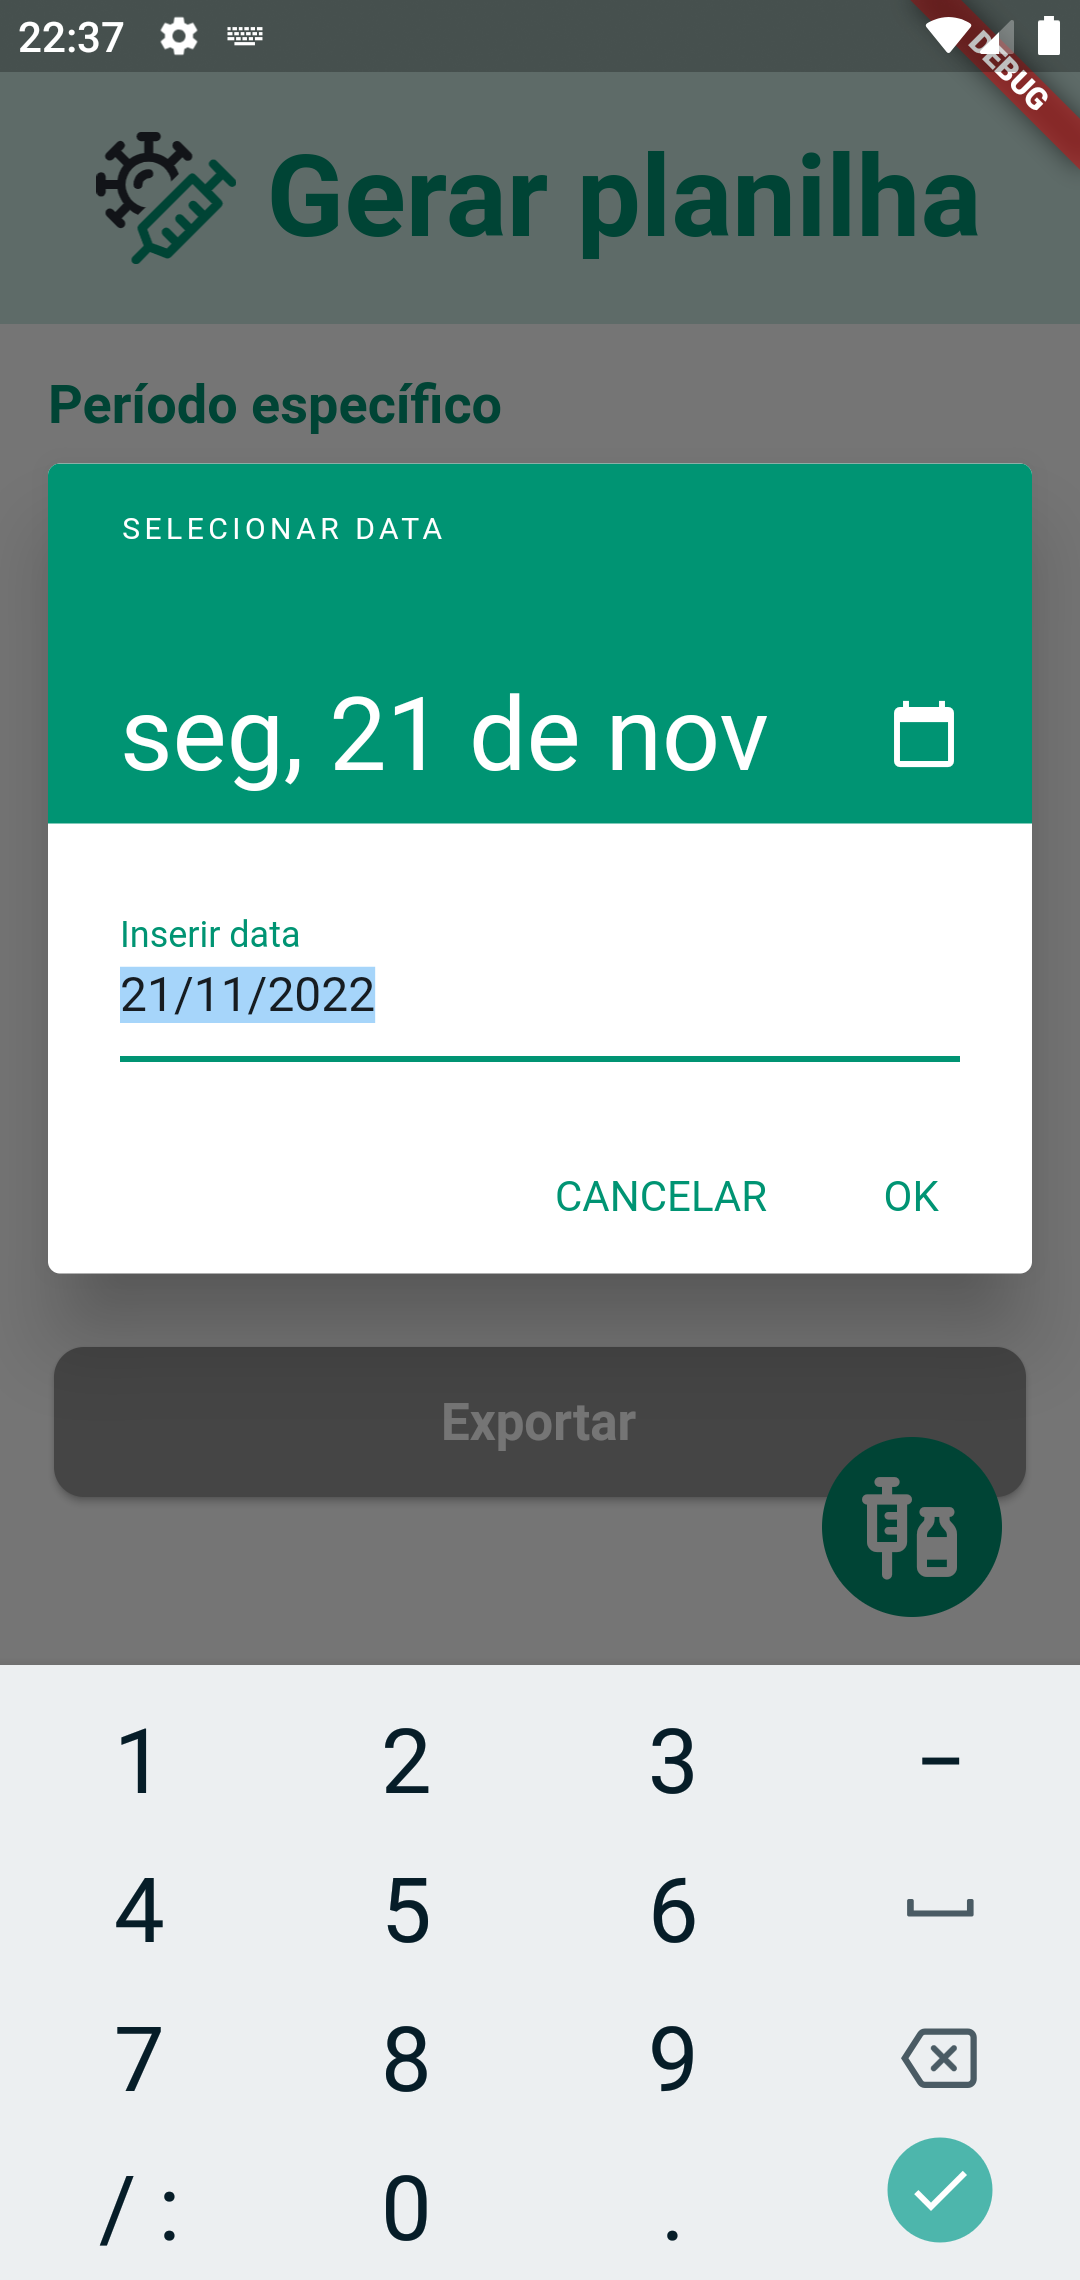
\includegraphics[width=0.29\columnwidth]{figuras/cap4/4_2_export_screen_2.png}}
            \qquad
          \subfloat[\textbf{Calendário 2 para escolha do período de exportação}]{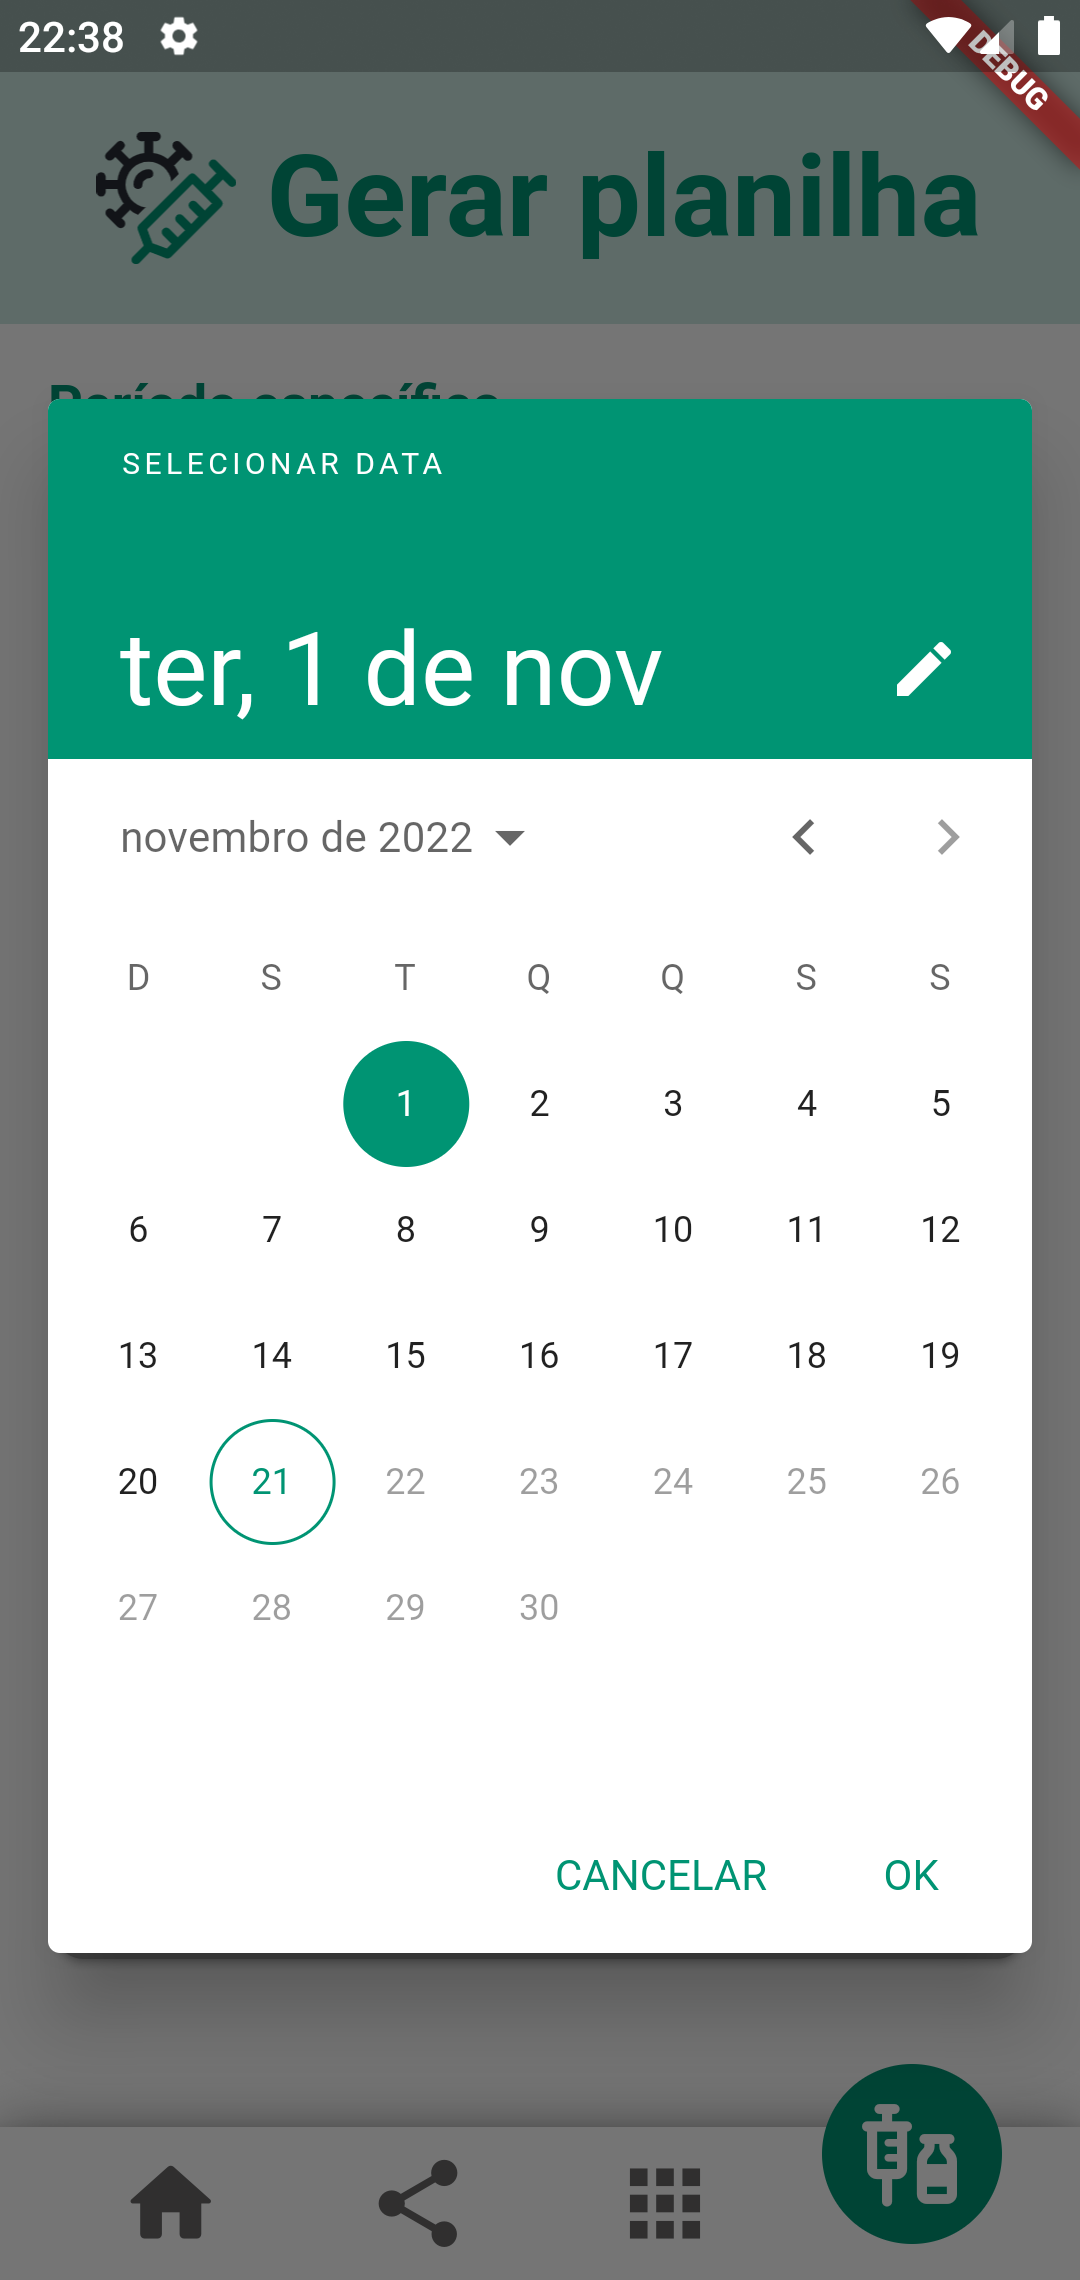
\includegraphics[width=0.29\columnwidth]{figuras/cap4/4_2_export_screen_3.png}}
    \caption[Fluxo de exportação da planilha de vacinação (parte 1)]{Fluxo de exportação da planilha de vacinação (parte 1)}
  % \fonte{Inserir autor aqui}
  
  \label{fig:export_flux_1}
\end{figure}

\begin{figure}[ht!]
  \centering
          \subfloat[Pop-up \textbf{para escolha entre abrir ou exportar a planilha}]{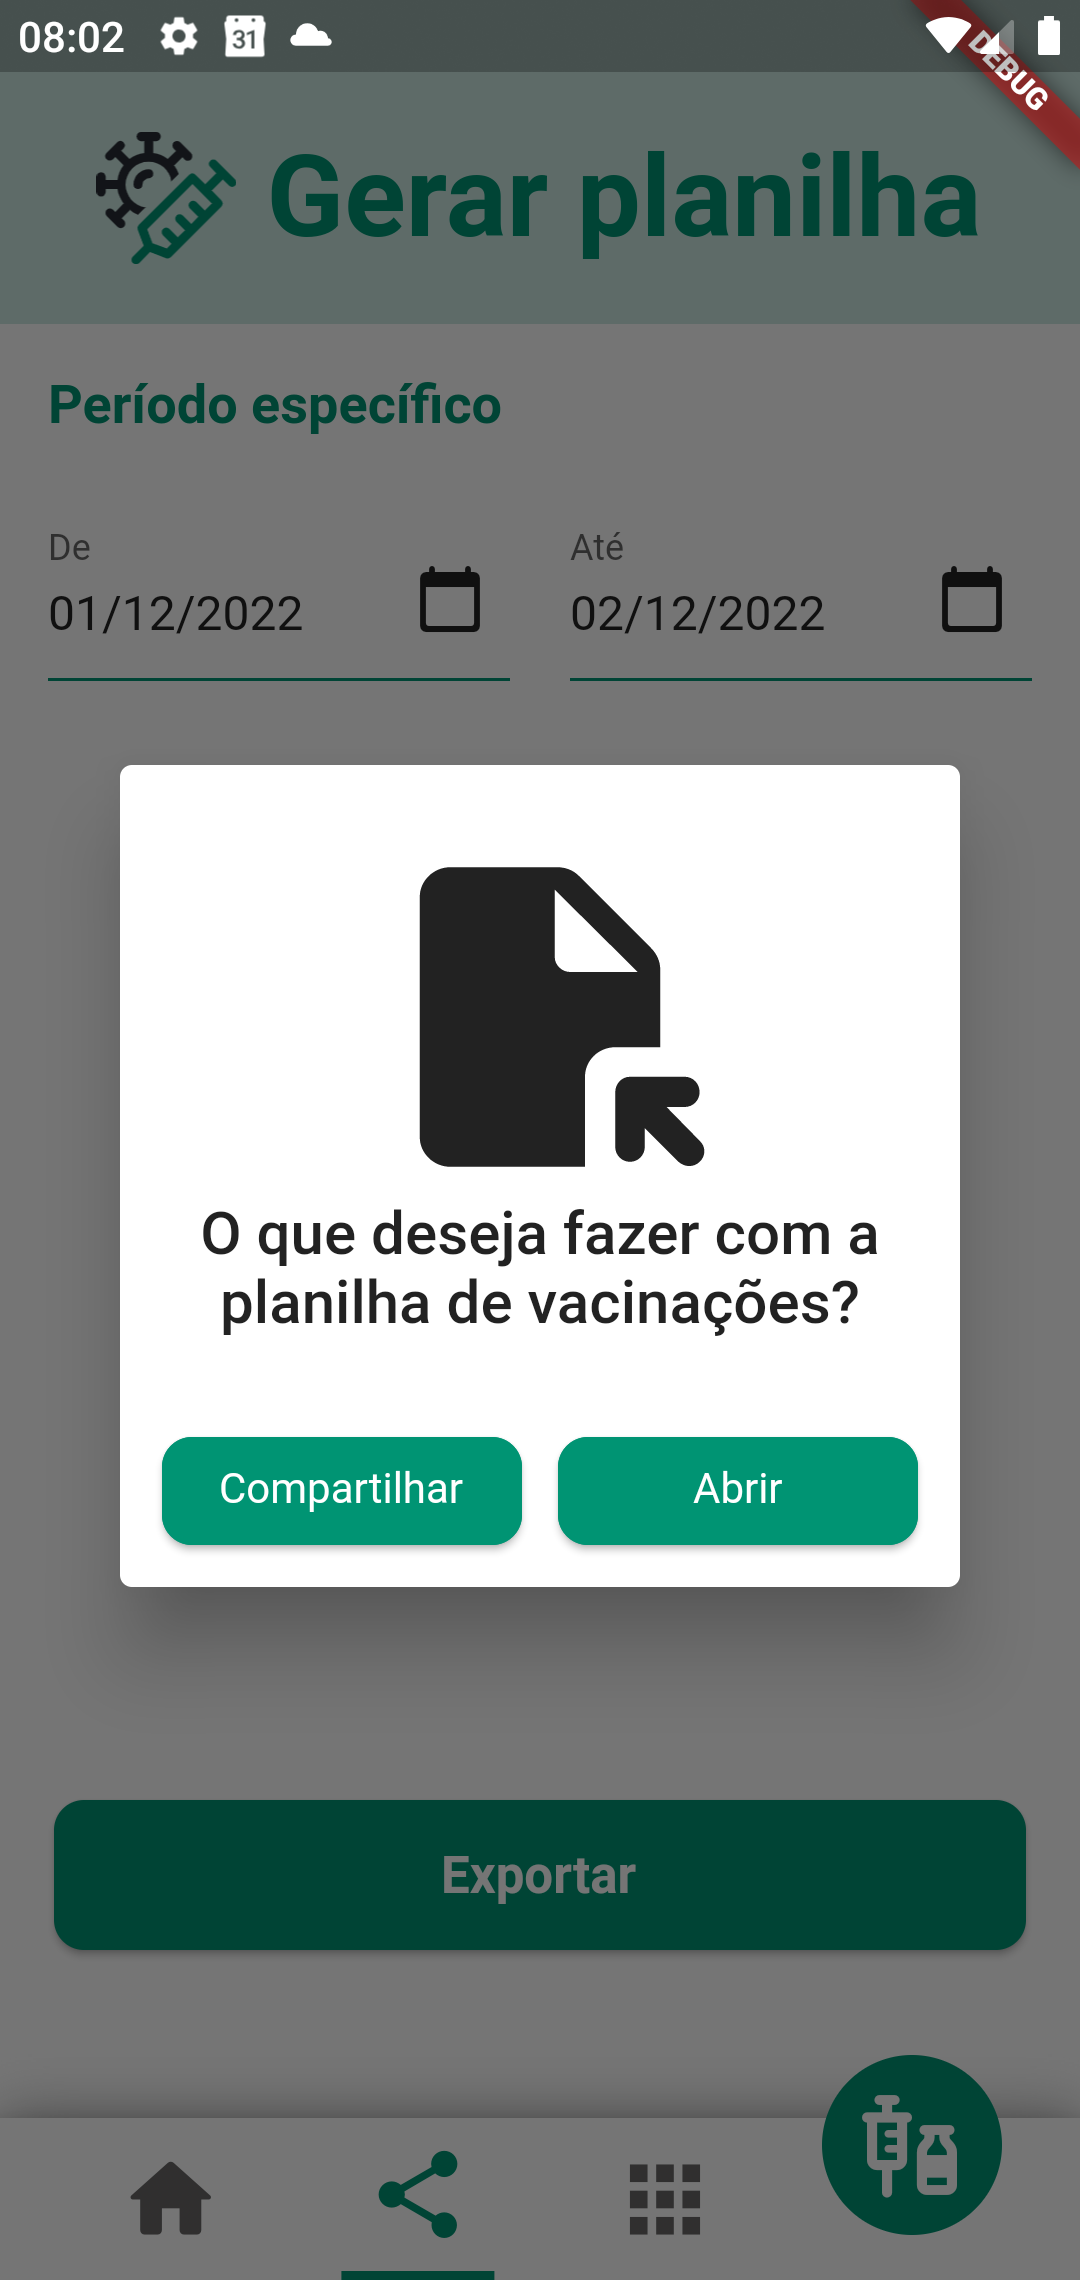
\includegraphics[width=0.29\columnwidth]{figuras/cap4/4_2_export_screen_5.png}}
            \qquad
          \subfloat[Janela do sistema \textbf{para escolha do aplicativo externo}]{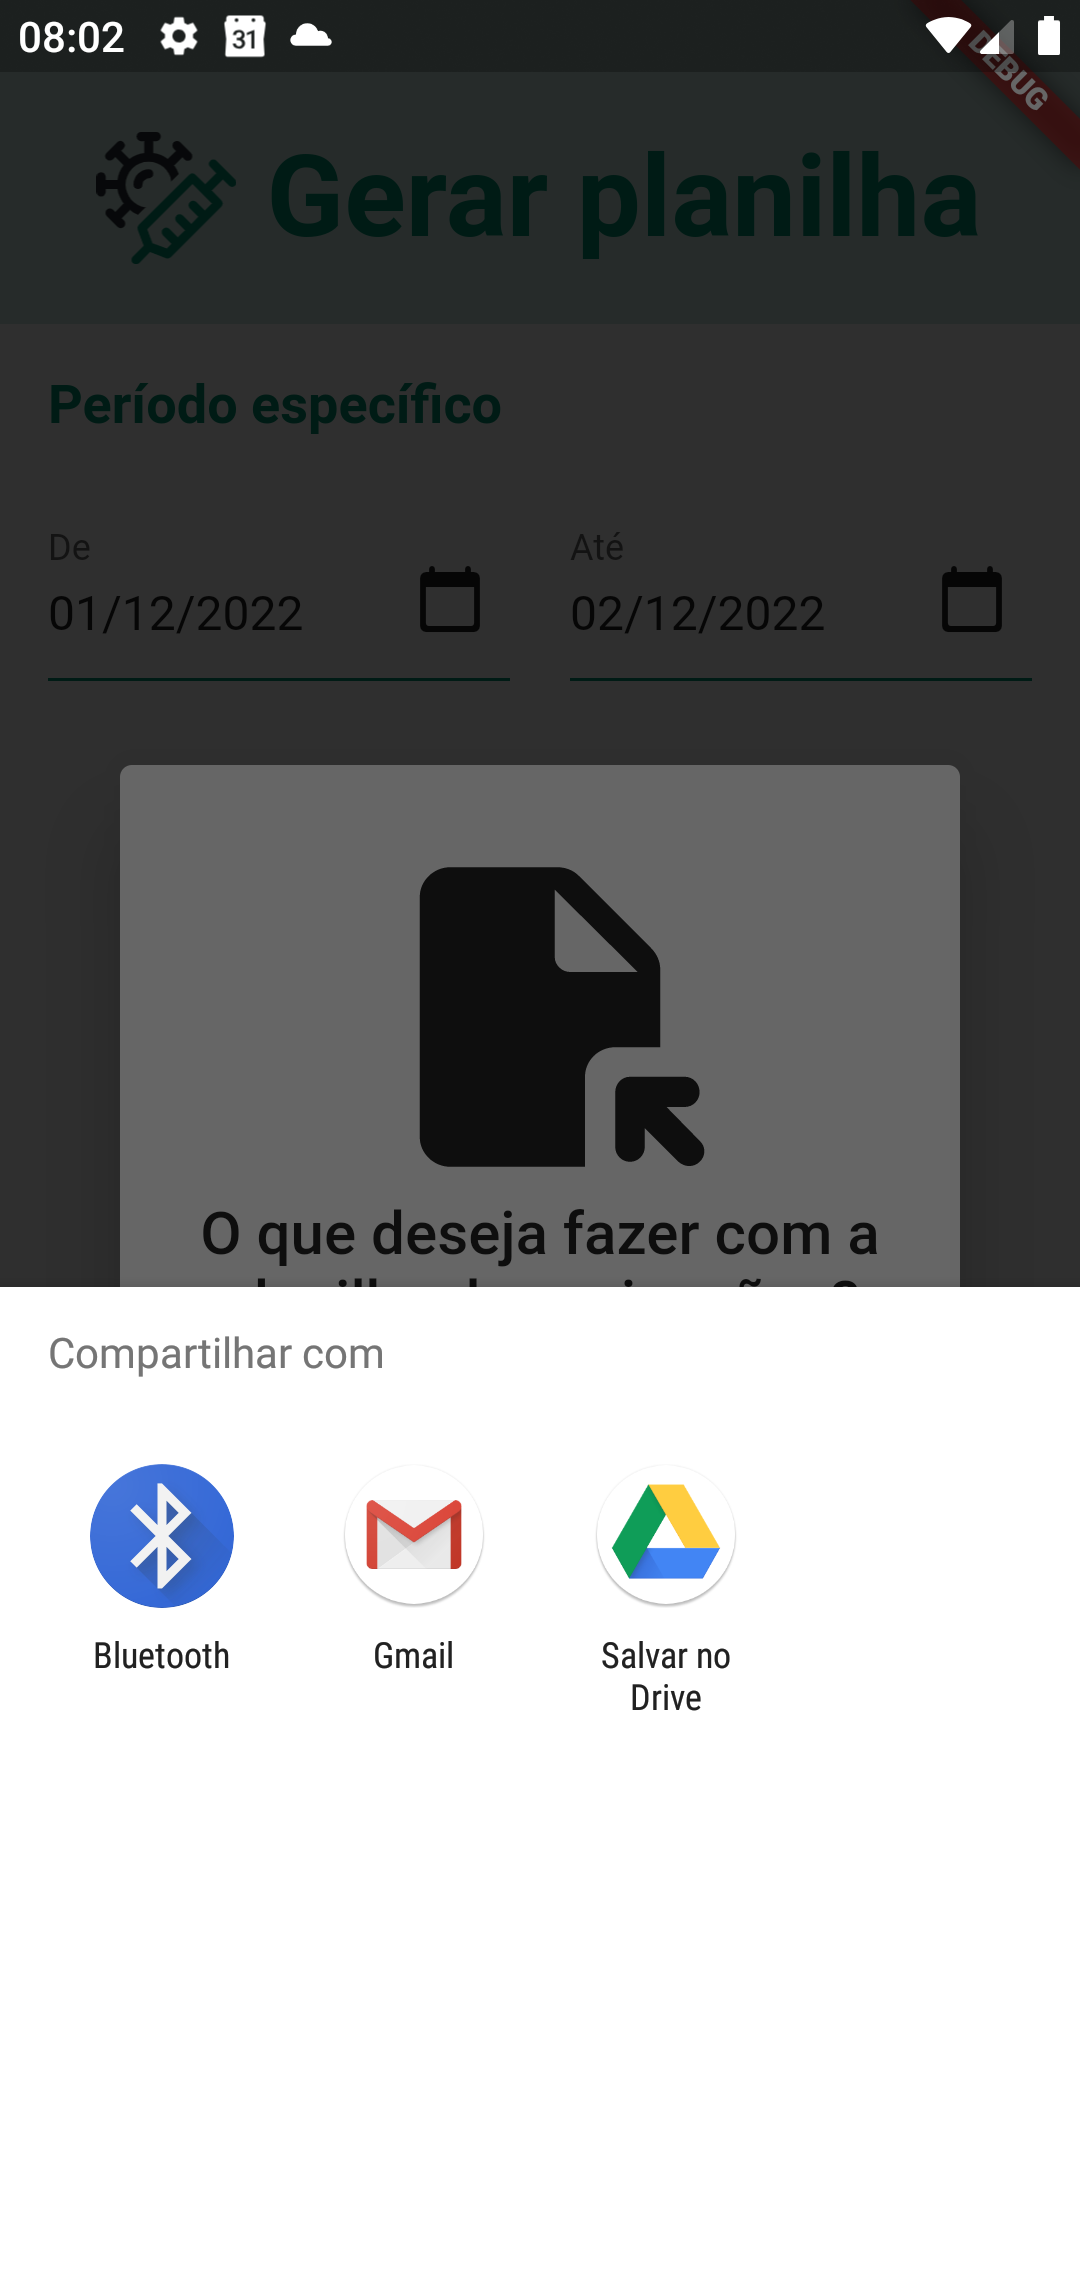
\includegraphics[width=0.29\columnwidth]{figuras/cap4/4_2_export_screen_6.png}}
    \caption[Fluxo de exportação da planilha de vacinação (parte 2)]{Fluxo de exportação da planilha de vacinação (parte 2)}
  % \fonte{Inserir autor aqui}
  
  \label{fig:export_flux_2}
\end{figure}

% \section{Testes de segurança}
% \label{cap5:Sec:TestesSeguranca}
% Aqui posso falar sobre a tentativa de adicionar dados inválidos.





